\label{sec:vbf-nonres}

In order to determine the non-resonant background, we fit  the sidebands of each of the BDT regions independently with an analytical function. The sidebands of the \Mbb{}  distribution of each BDT region are shown in Fig. \ref{fig:vbf-mbb_sidebands}. %An alternative approach  using a control region and a linear transfer factor to relate the control region shape to the signal regions is documented in Appendix~\ref{sec:vbf-app-oldfitbkgds}.  However, due to concerns about the validity of the approach, documented in Appendix~\ref{sec:vbf-app-LinearityTest}, the more conservative approach of independent fits is taken here.  

\begin{figure}[htbp]
  \centering
 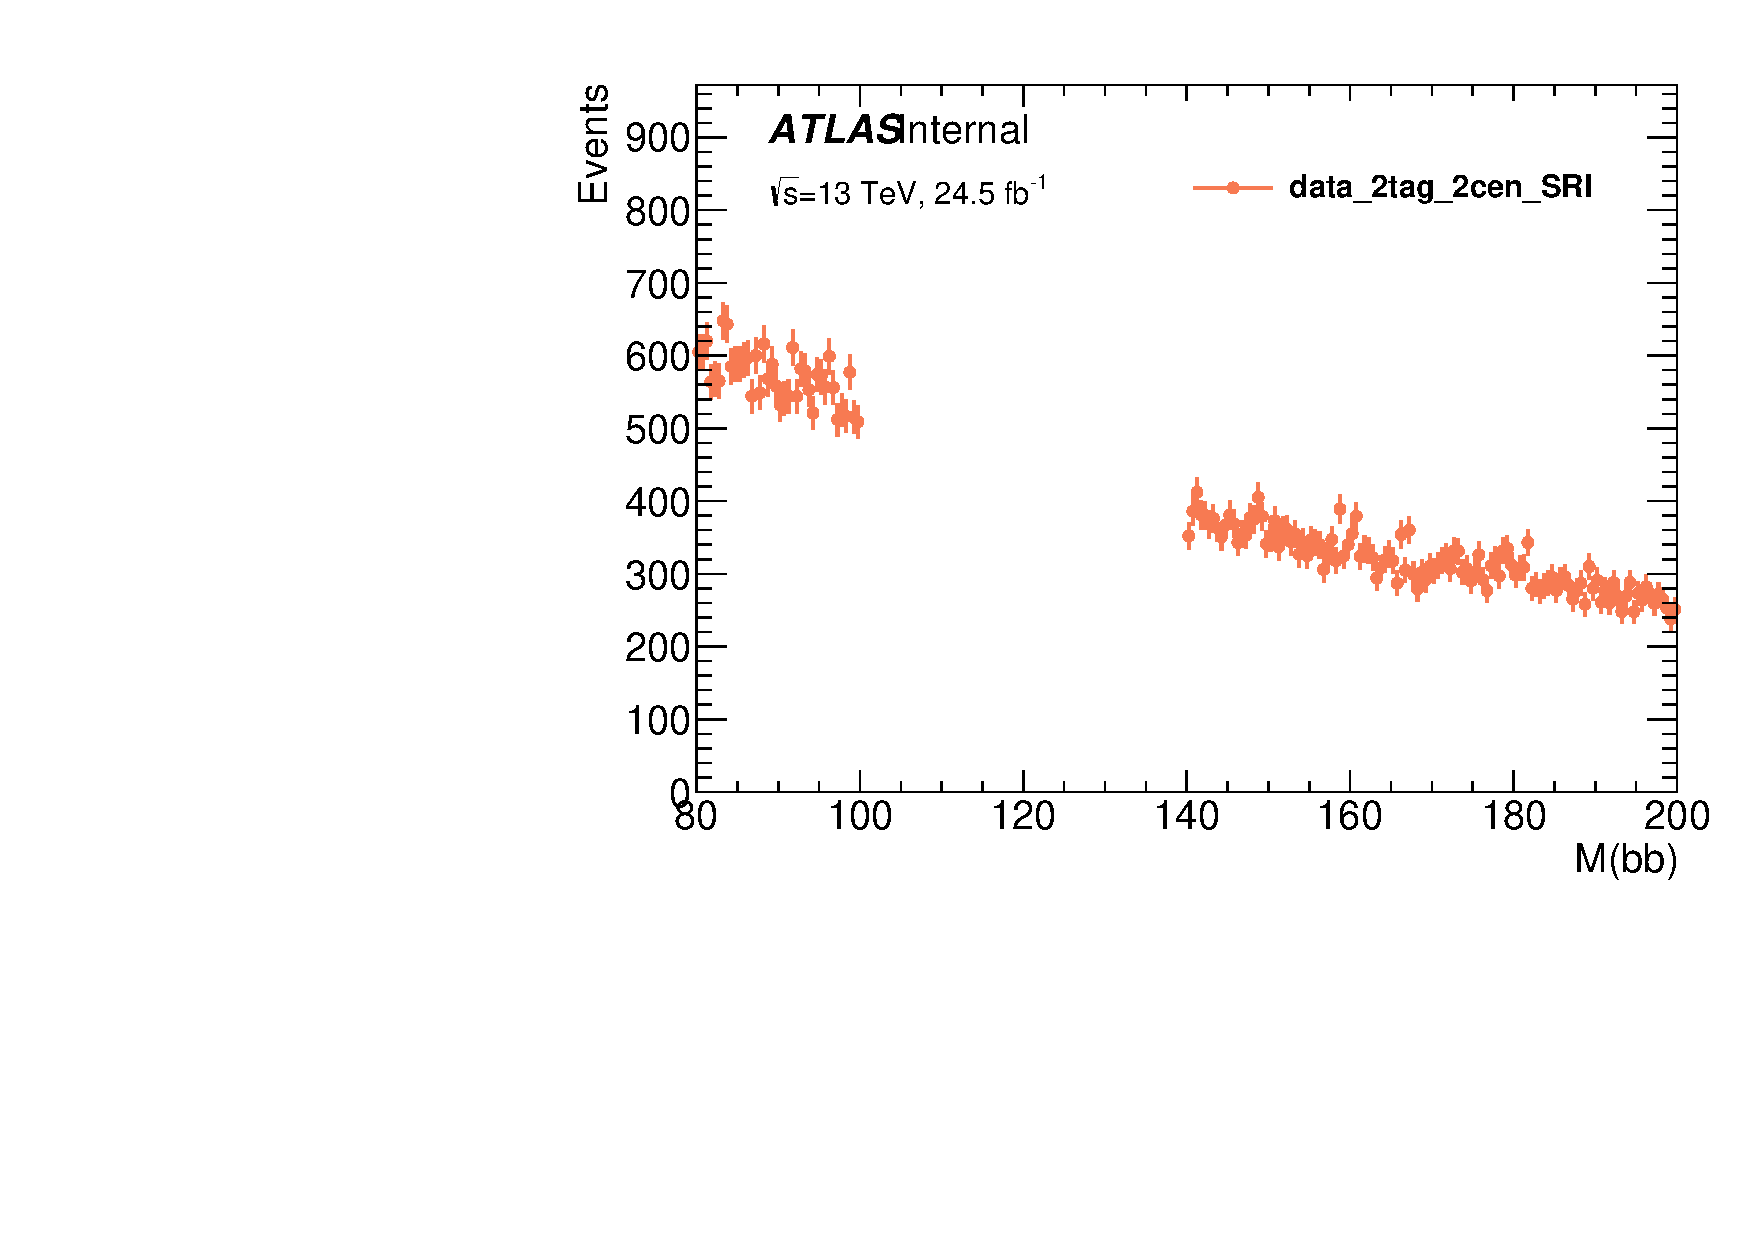
\includegraphics[width=0.45\textwidth]{figures/VBF/Mbb_SRI_2cen.pdf}
 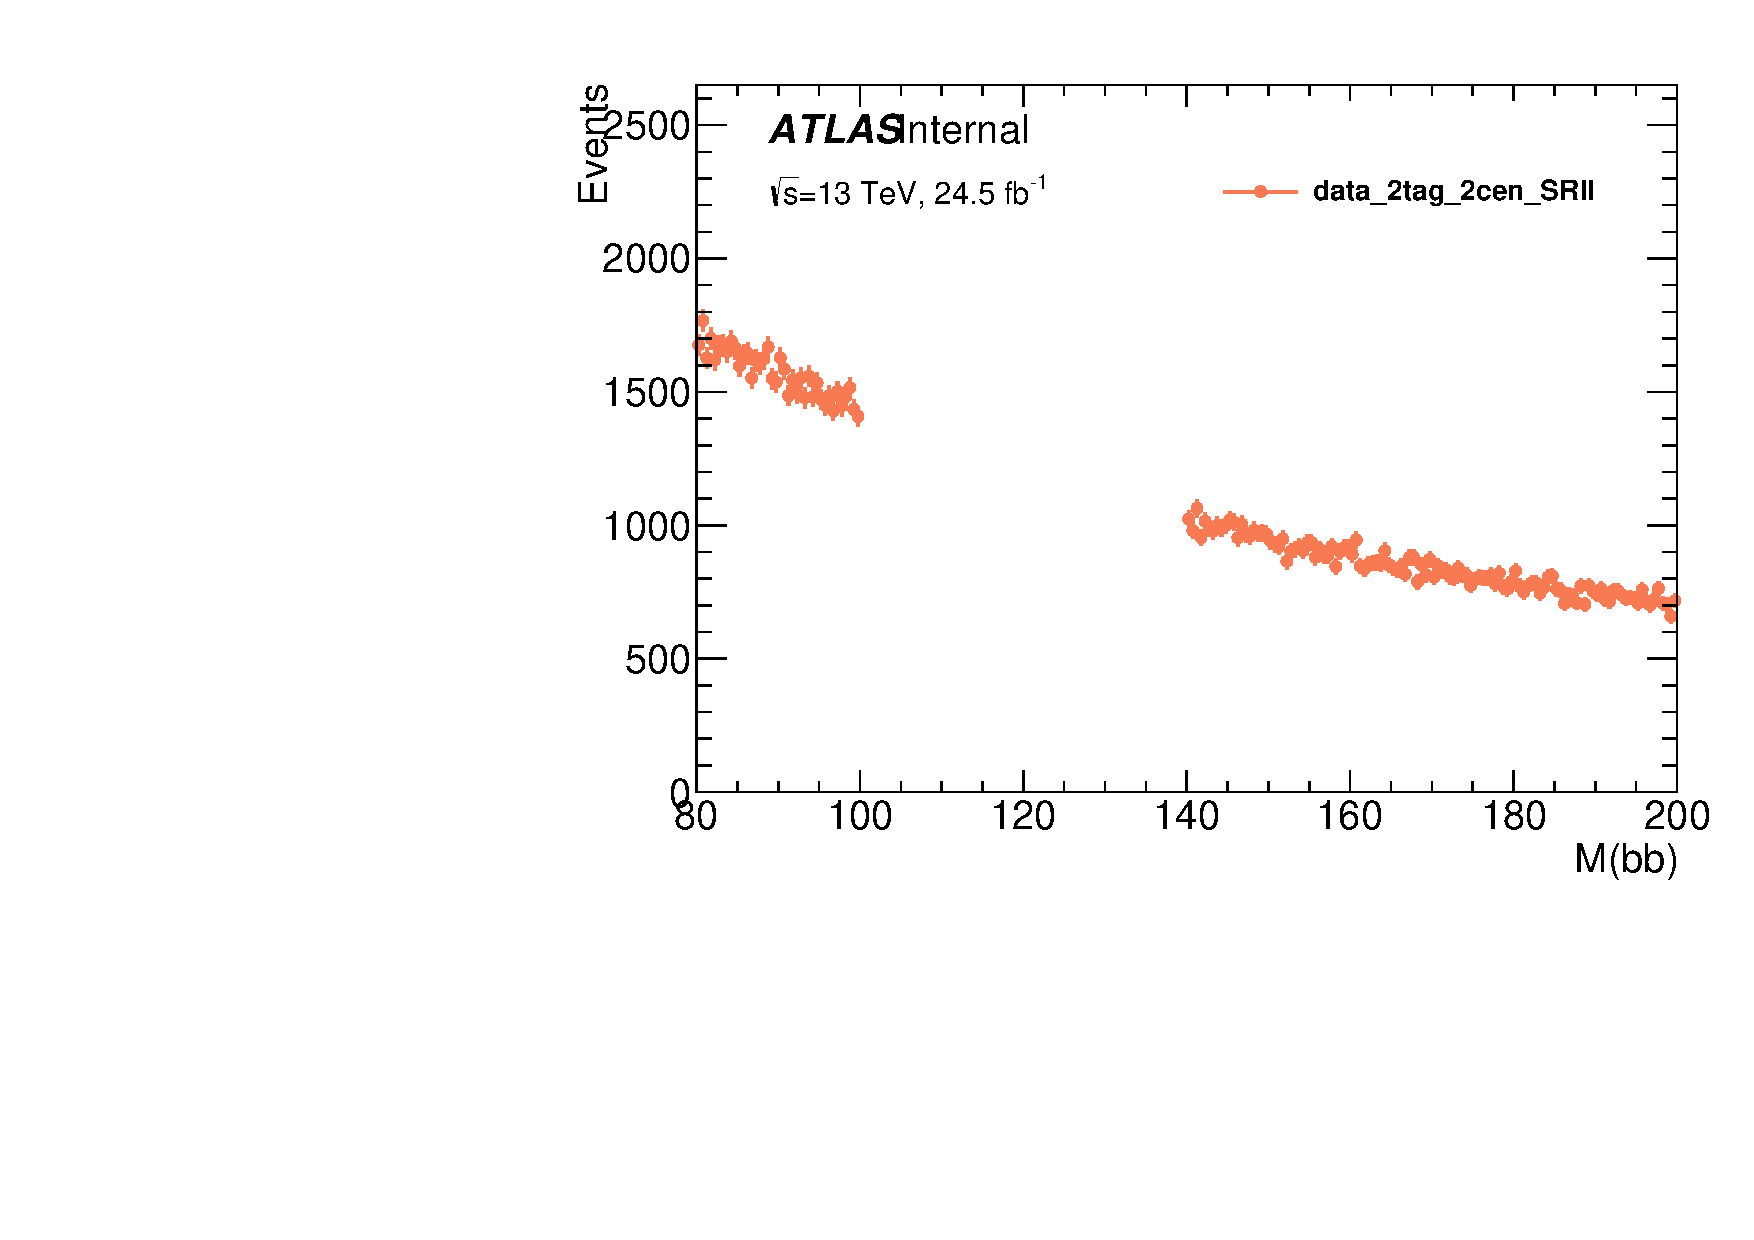
\includegraphics[width=0.45\textwidth]{figures/VBF/Mbb_SRII_2cen.pdf}\\
 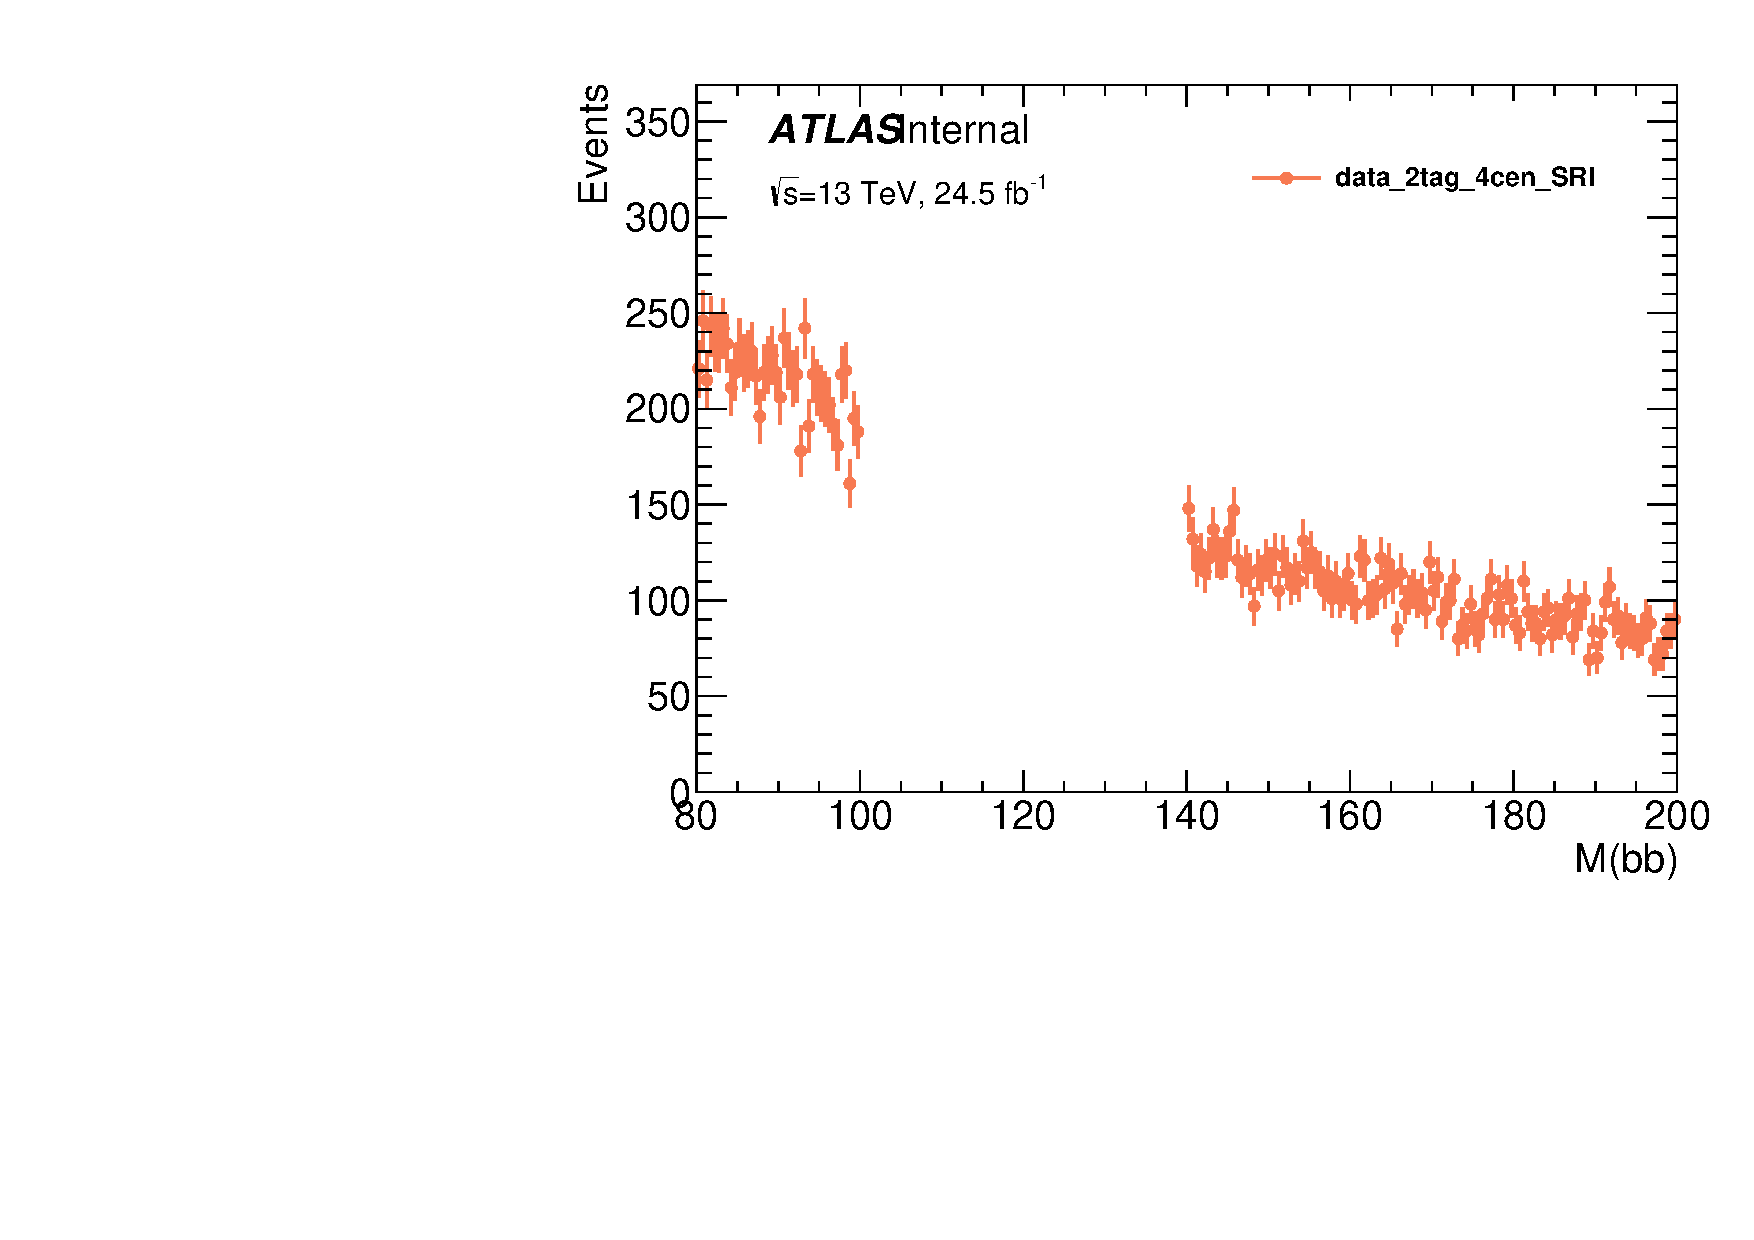
\includegraphics[width=0.45\textwidth]{figures/VBF/Mbb_SRI_4cen.pdf}
 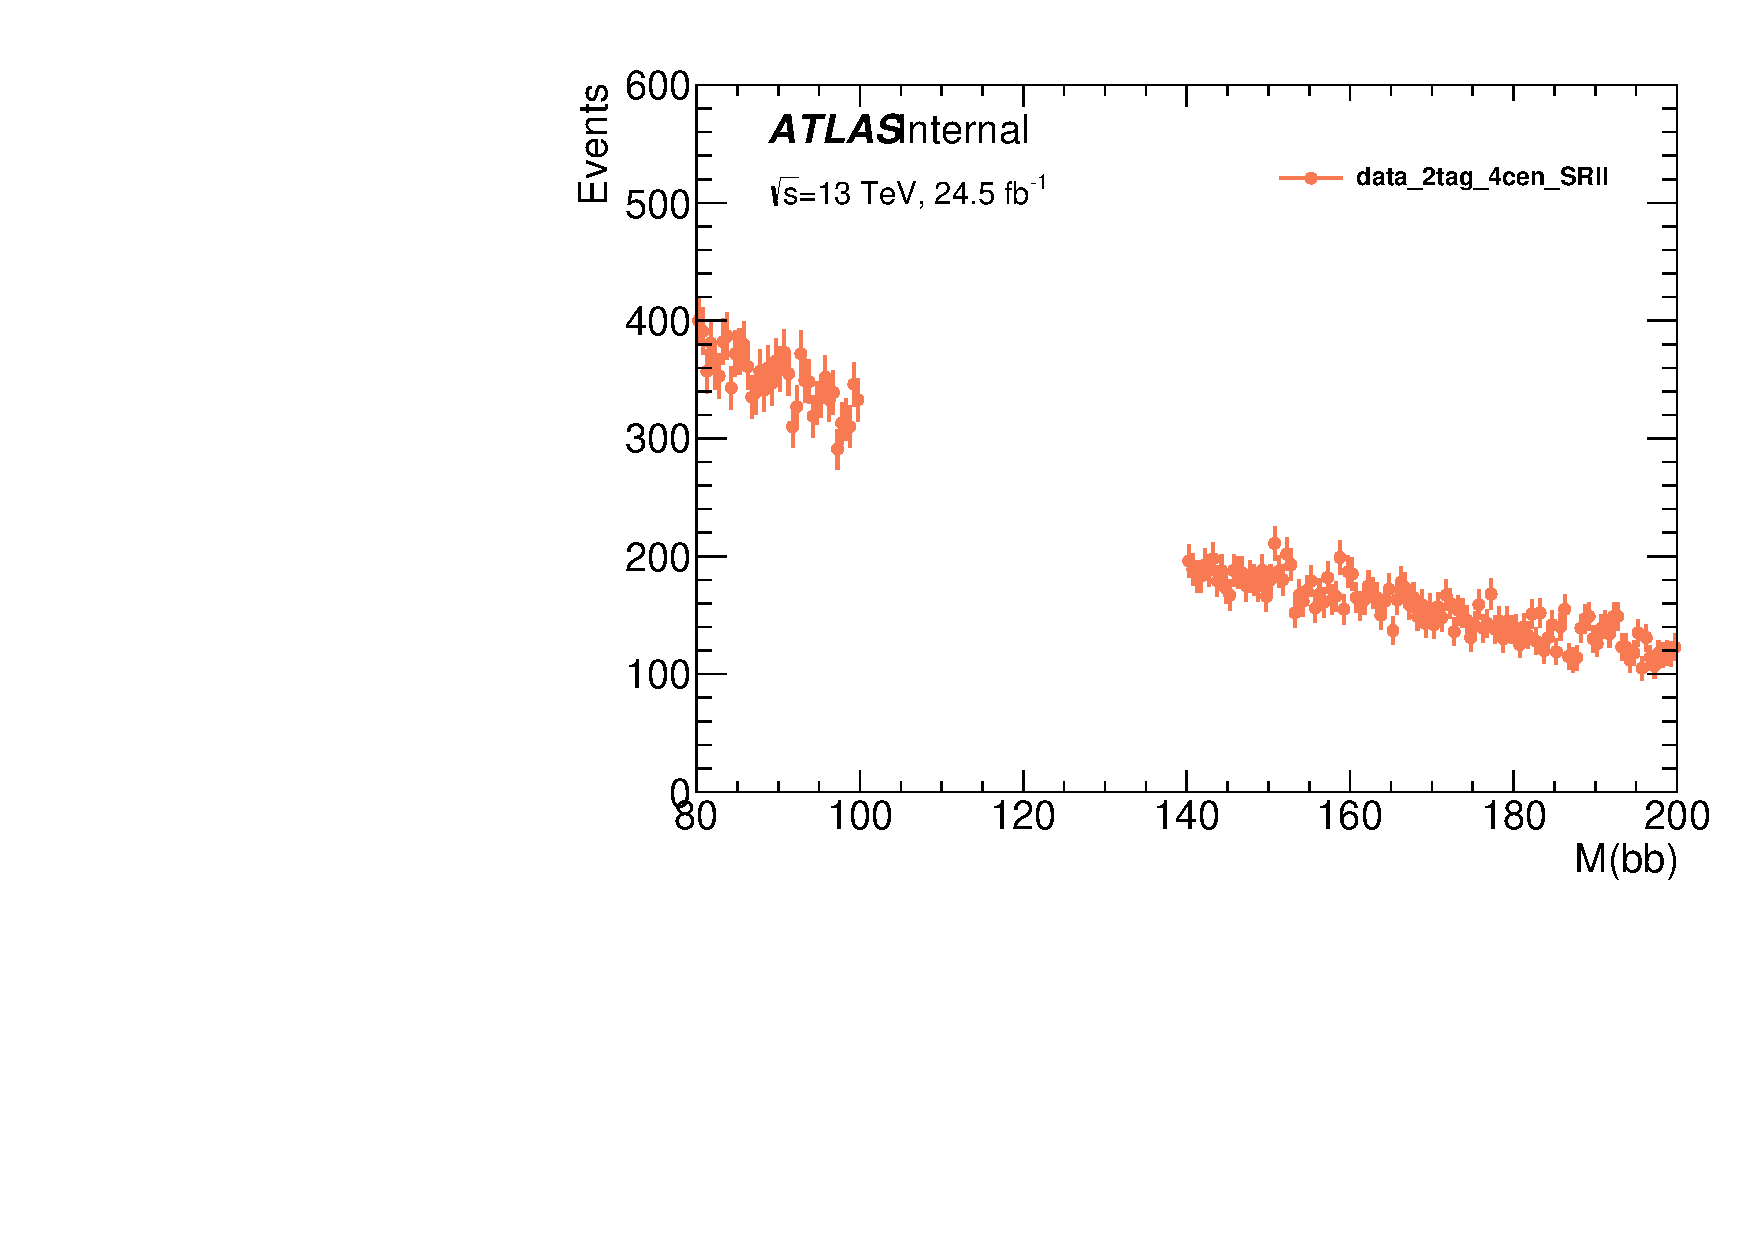
\includegraphics[width=0.45\textwidth]{figures/VBF/Mbb_SRII_4cen.pdf}\\
 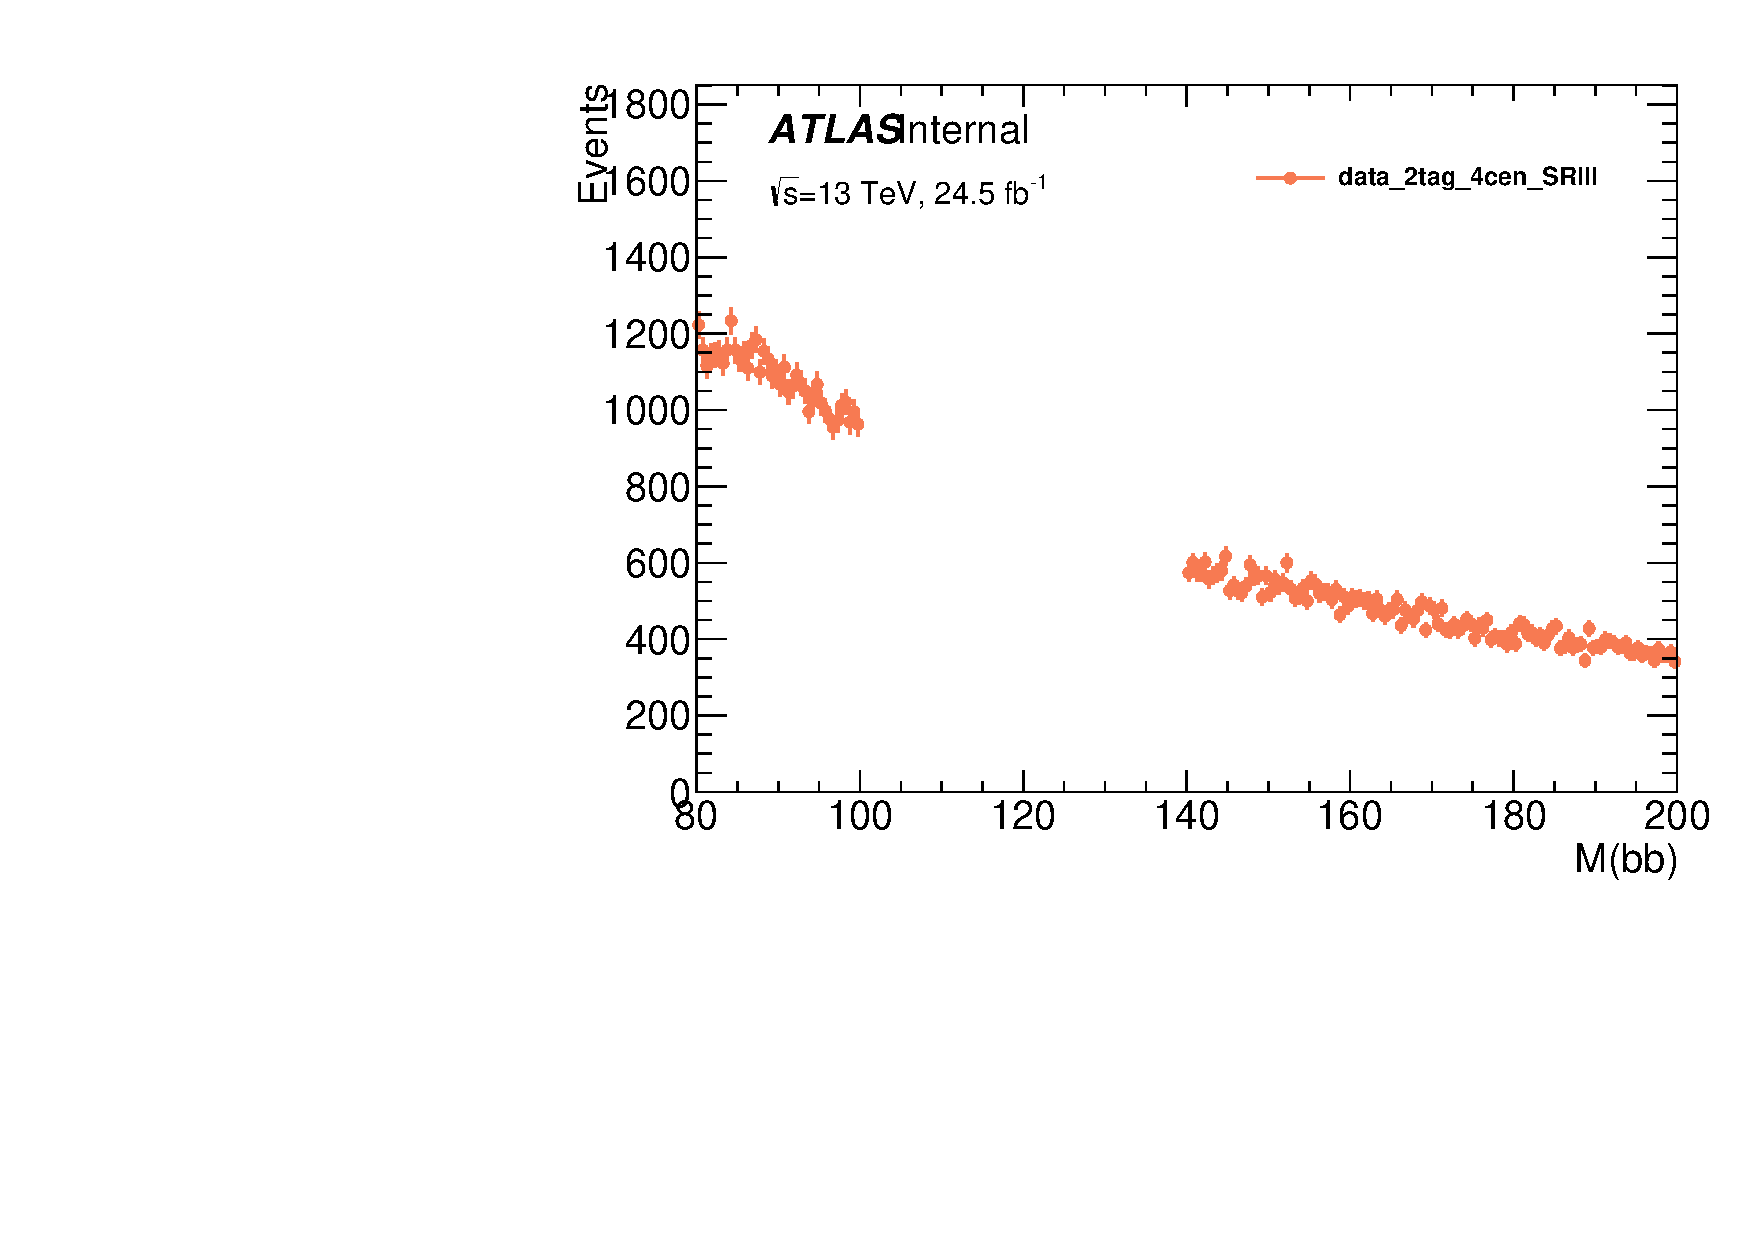
\includegraphics[width=0.45\textwidth]{figures/VBF/Mbb_SRIII_4cen.pdf}
 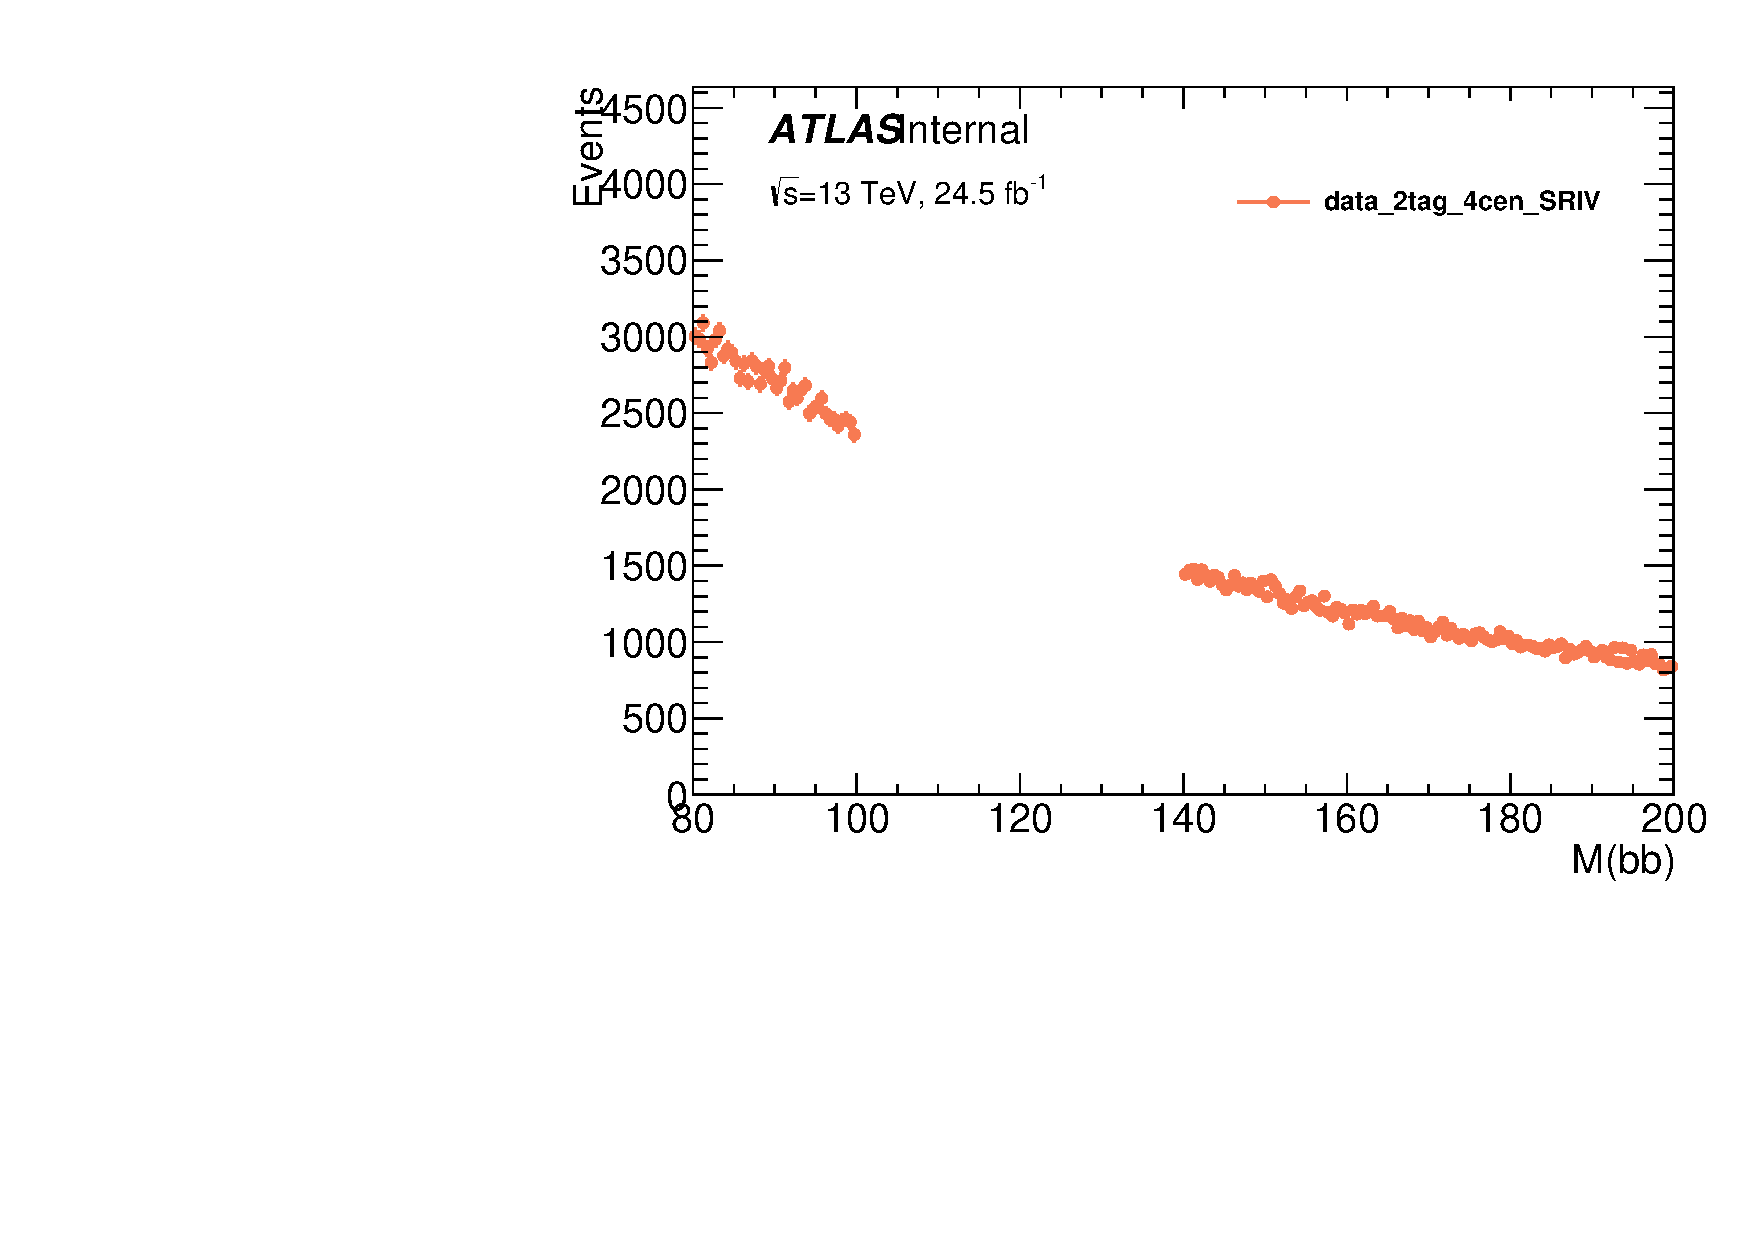
\includegraphics[width=0.45\textwidth]{figures/VBF/Mbb_SRIV_4cen.pdf}\\
\caption{\Mbb{} shapes of all BDT regions in sidebands} 
  \label{fig:vbf-mbb_sidebands}
\end{figure}


Several function families are considered and tested. The primary family of functions considered is that of the Bernstein polynomials listed in Equation~\ref{eq:bernstein}, which were
used successfully in the previous iteration of this analysis. The product of Bernstein and exponential functions, as well as the sum of exponentials, were used as the alternative functions for background description.
The functions chosen are required to pass two conditions. Among the candidates satisfying the conditions above, the function with the smallest number of degrees of freedom is chosen.

\begin{itemize}
\item 
Compatibility: The function must be statistically  compatible with the sidebands of the \Mbb{} distribution in the signal regions, where the Higgs mass range $100<\Mbb<140$ GeV is ignored. The compatibility criterion is defined as $P(\chi^2)>0.05$ and $P(F-\rm{test})>0.05$,  where the $\chi^2$ and $F-\rm{test}$ probabilities are considered, respectively. The $F-\rm{test}$ is performed with respect to the $n+1$ order function.  Only statistical errors are considered in these fits.  Among the candidates satisfying the conditions above, the function with the smallest number of degrees of freedom is chosen. For this study, the \zjets{} component is included in the fit,  normalized to the SM prediction.

\item Spurious Signal:  The lowest order function that satisfies compatibility condition, $f_{B}$, is tested against the the lowest order functions in an alternative truth model, $f_{A}$, that also satisfies the compatibility condition, to derive the spurious signal size \cite{CMS-HIG-12-028}. This is a standard approach used for similar analysis. Although in the future this approach needs better understanding if it double counts partial statistical uncertainty of data, we adopt this apporach to be conservative in estimating uncertainty. We build pseudo data from $f_{A}$, where the parameters of the function are derived from the fit to the sidebands in each signal region.  We then fit the distribution with $f_{B}$ plus $\mu_{sp}$ times the signal template. The measured  apparent signal size needs to be less than $50\%$ of the actual signal size. If this test fails, the the next order function satisfying the compatibility condition is tested.  The \zjets{} component is not included in the pseudo data.

\end{itemize}


The $\chi^2$ values and probabilities and $F-\rm{test}$ probabilities are summarized in Tables~\ref{tab:chi2-2cen} through~\ref{tab:f-test}. The $\chi^2$ test criteria are met for the O(2) Bernstein function in all regions, except in 
SR IV of the \fourcentral channel where we need at least an O(3) Bernstein function. The $F$-test is passed for functions which pass the $\chi^2$ criterion in all channels and regions.

The spurious signal fits are given in Tables~\ref{tab:spurious-test-2cen} and~\ref{tab:spurious-test-4cen}, which additionally show which functions are used as the alternative truth models. In most regions the O(3) Bernstein polynomial satisfies the spurious signal criterion. Note that our choice of background function minimizes the potential bias in trade of variance, i.e. the higher order functional forms yield larger uncertainty.

To satisfy all of the criteria, we choose an O(3) Bernstein function for the \twocentral channels, as well as for all SRs of the \fourcentral channel except SR IV which uses O(4).  


%\begin{figure}[htbp]
%  \centering
% 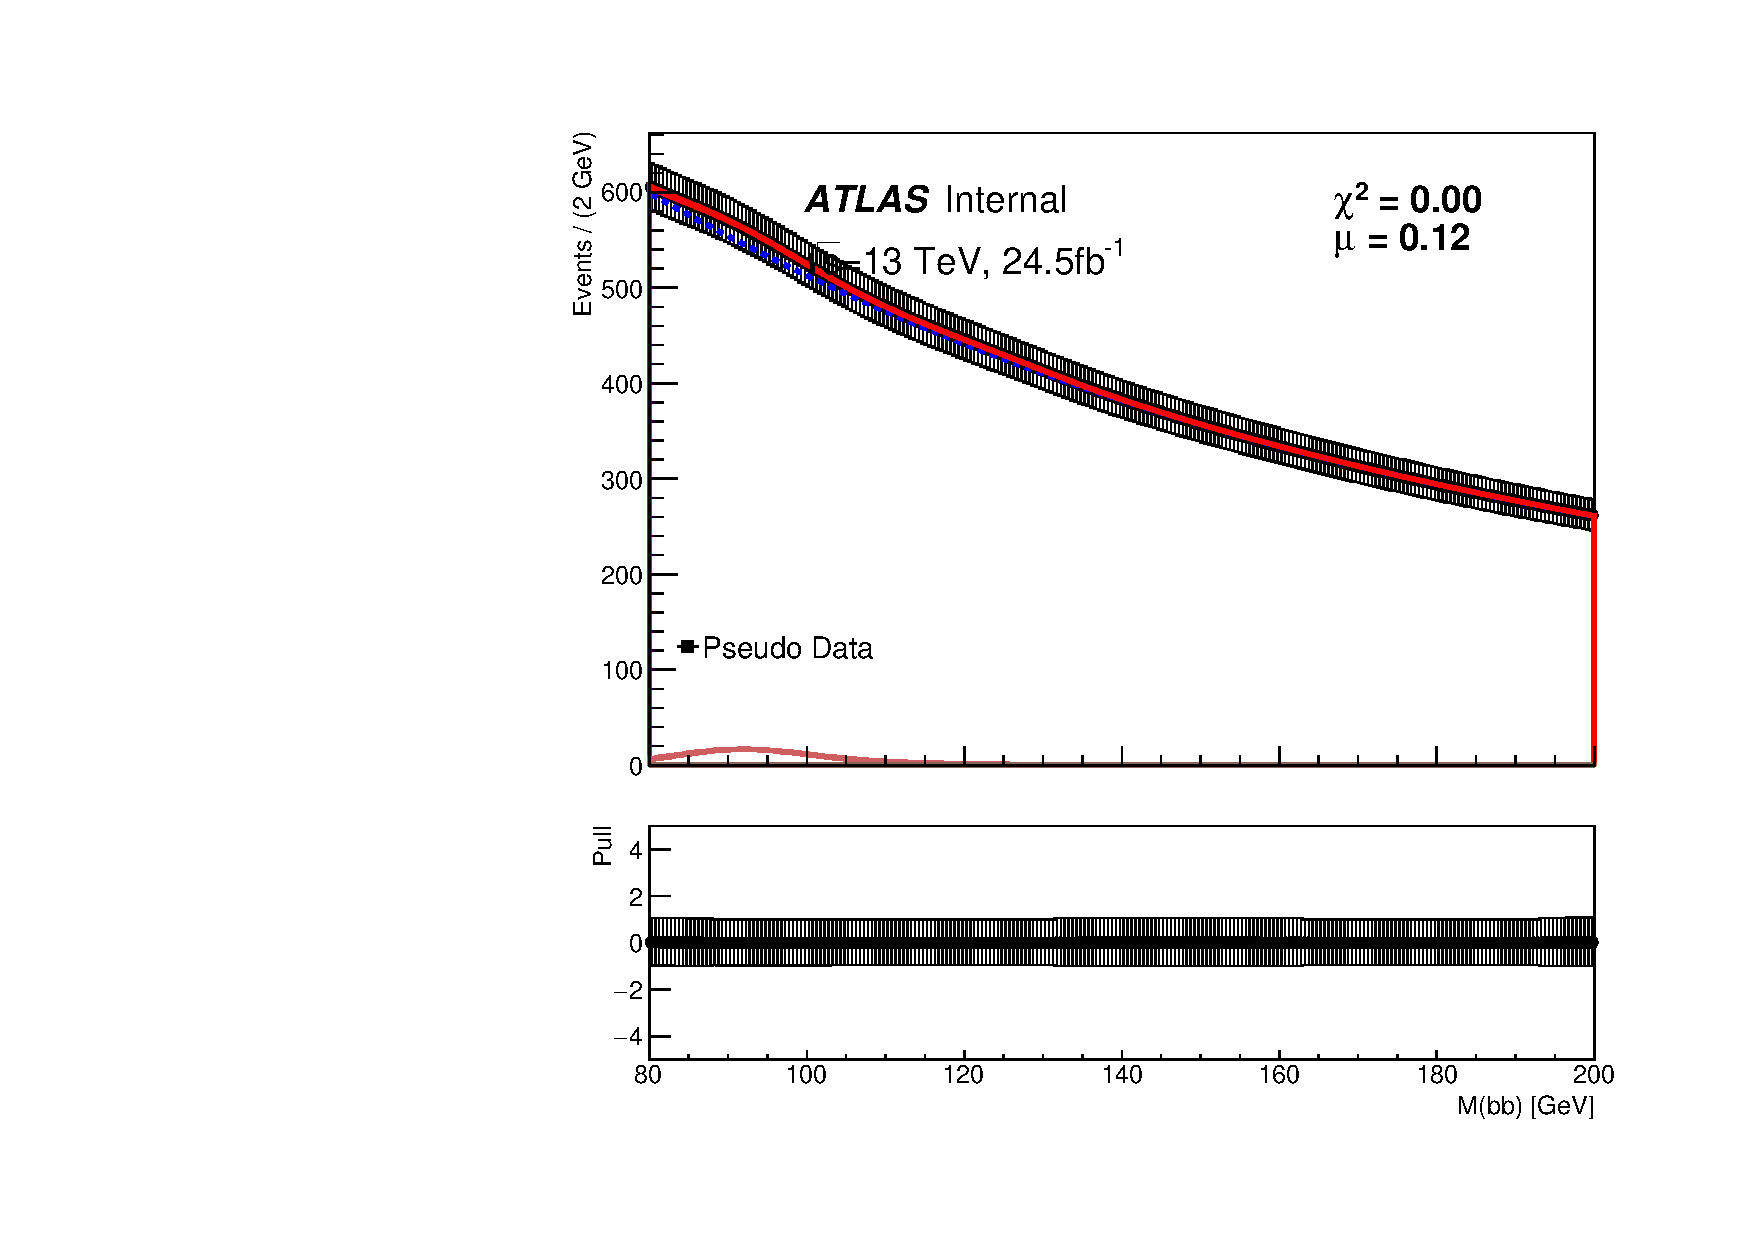
\includegraphics[width=0.24\textwidth]{figures/VBF/Spurious_ExpoO2_testVBF_ICHEP_2cen_SRI.pdf}
% 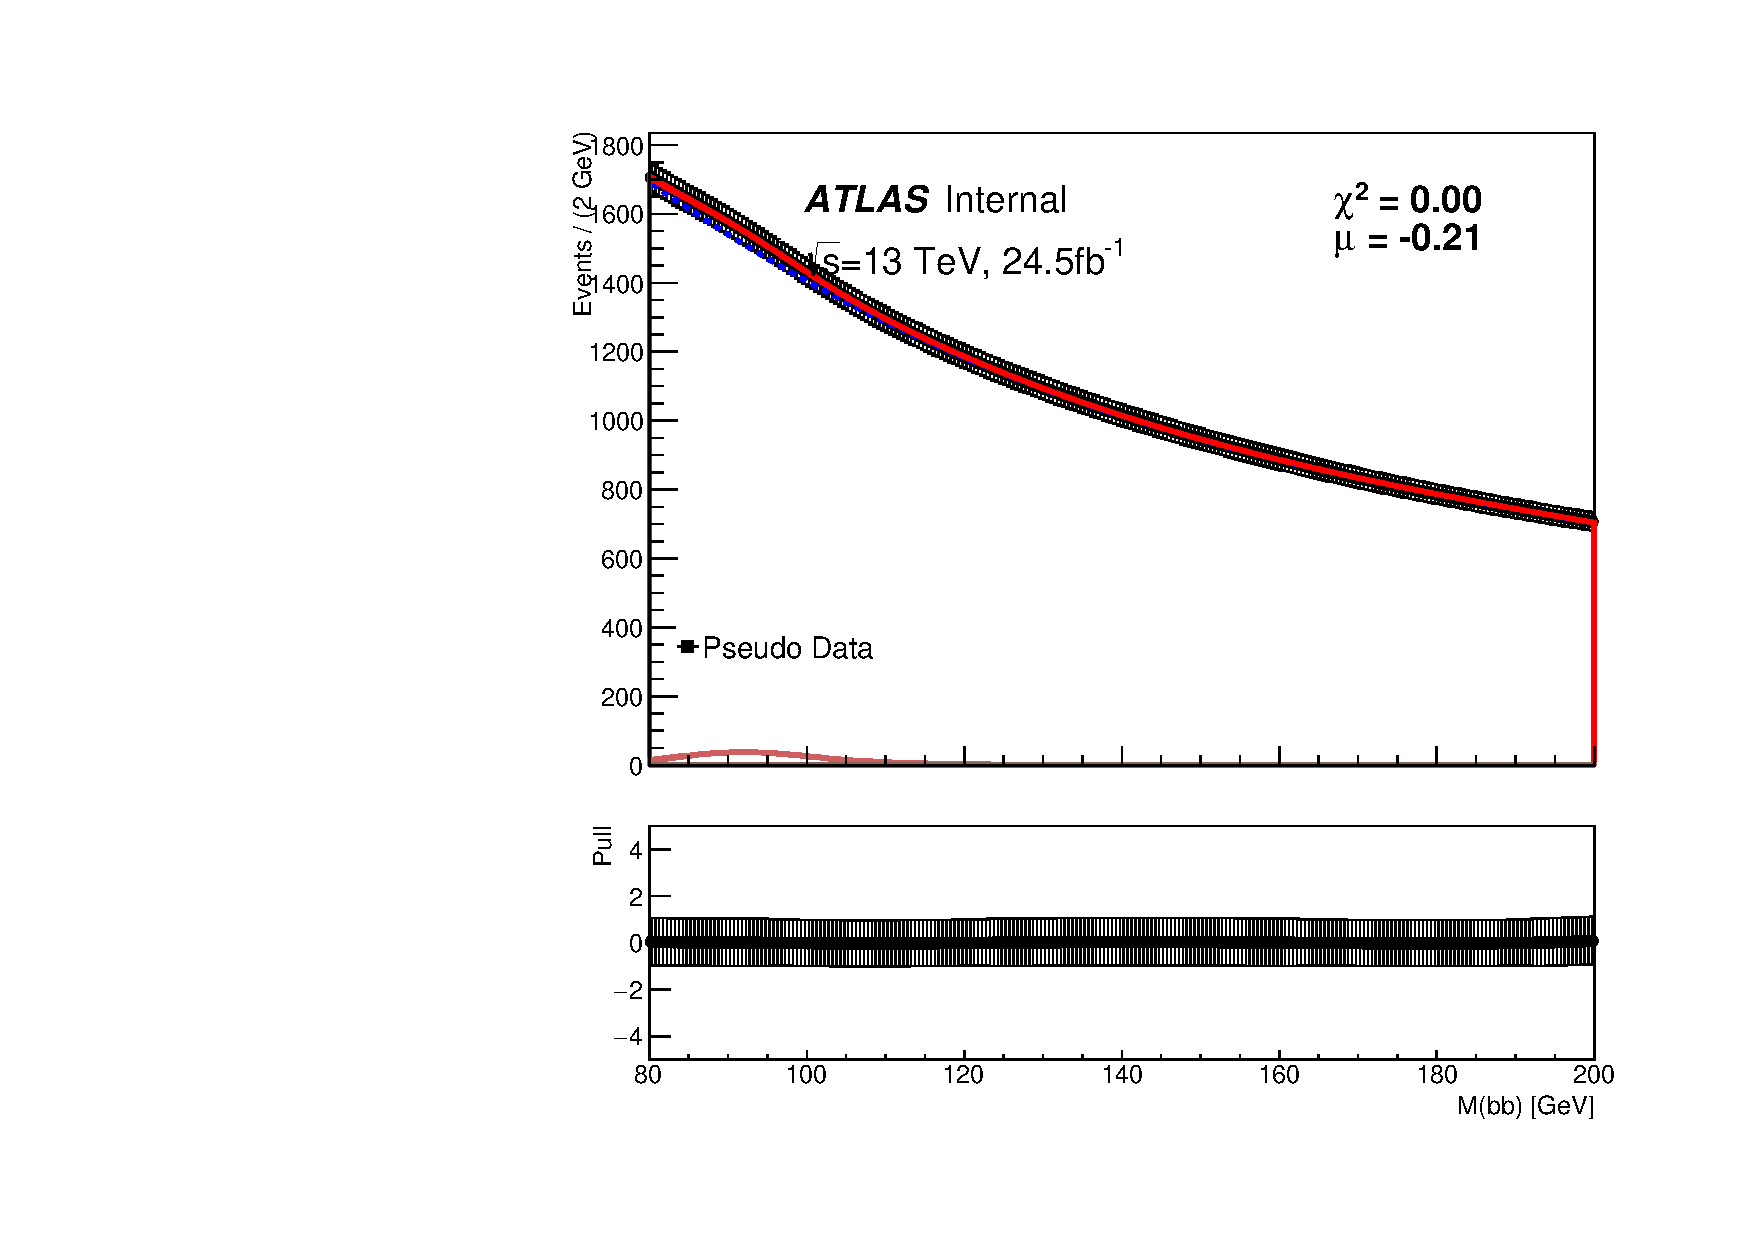
\includegraphics[width=0.24\textwidth]{figures/VBF/Spurious_ExpoO2_testVBF_ICHEP_2cen_SRII.pdf}\\
% 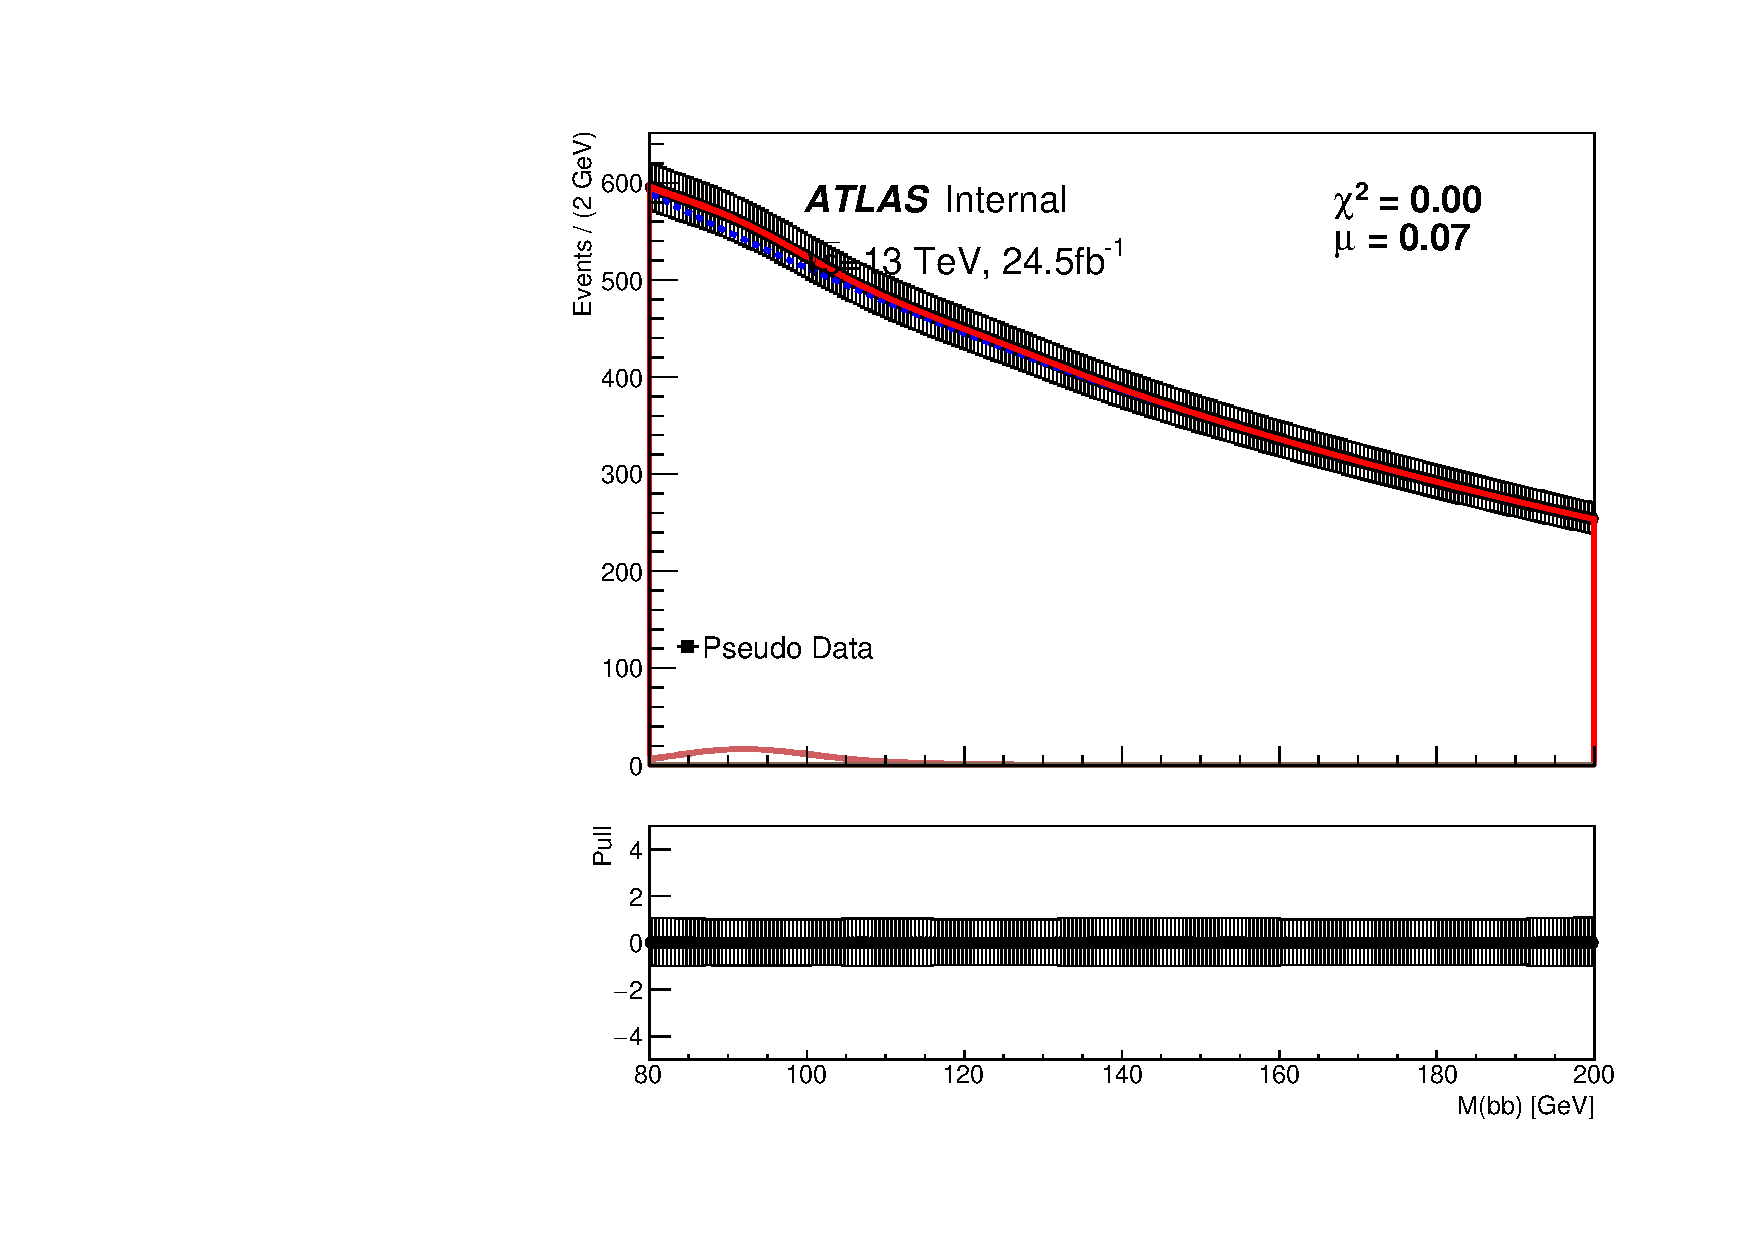
\includegraphics[width=0.24\textwidth]{figures/VBF/Spurious_SExpoO2_testVBF_ICHEP_2cen_SRI.pdf}
% 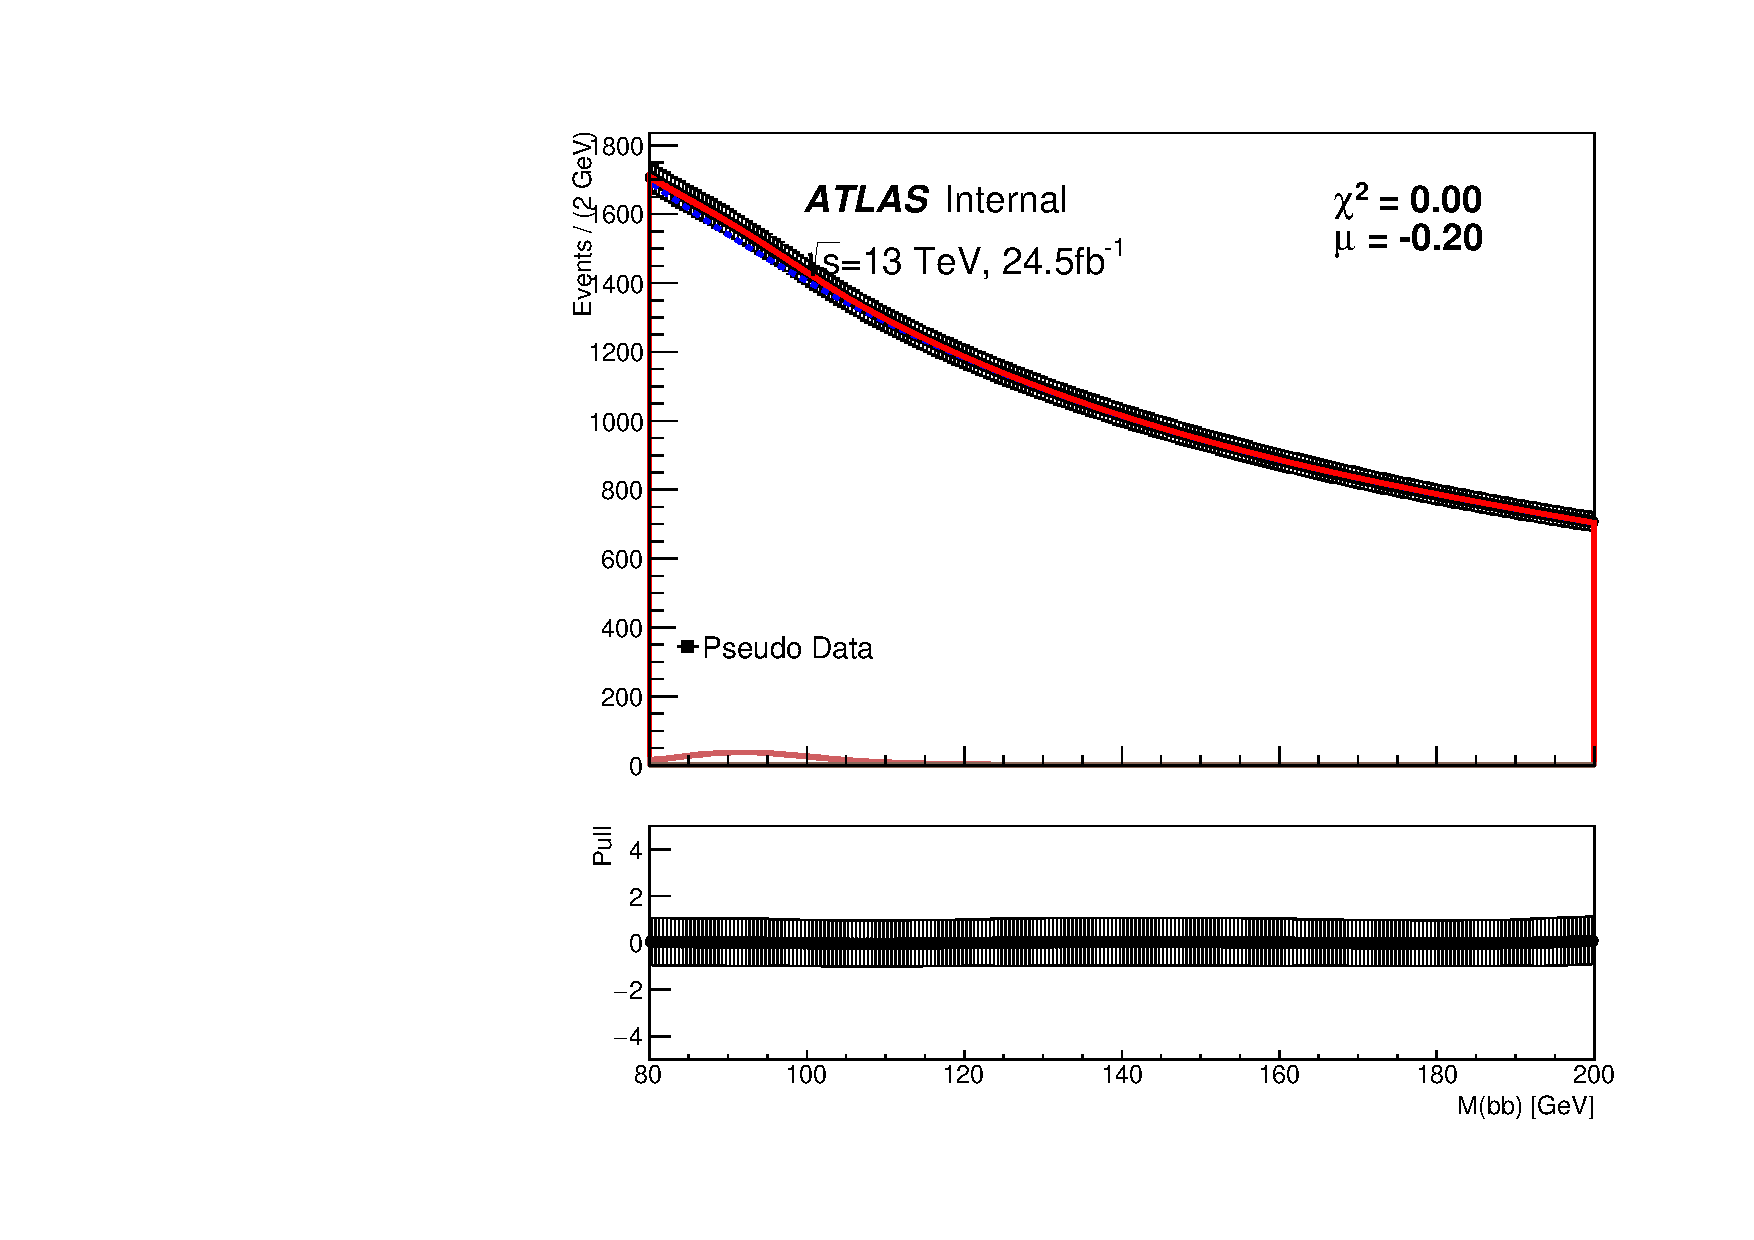
\includegraphics[width=0.24\textwidth]{figures/VBF/Spurious_SExpoO2_testVBF_ICHEP_2cen_SRII.pdf}\\
%\caption{Spurious signal fit for \twocentral channel for SR I to SR II (from left to right). The best Bernstein background models are tested against alternative truth models Expo*Bernstein O(2) (top) and Sum of Expo O(2) (bottom).}
%  \label{fig:vbf-Fit_SP_2cen}
%\end{figure}
%
%\begin{figure}[htbp]
%  \centering
% 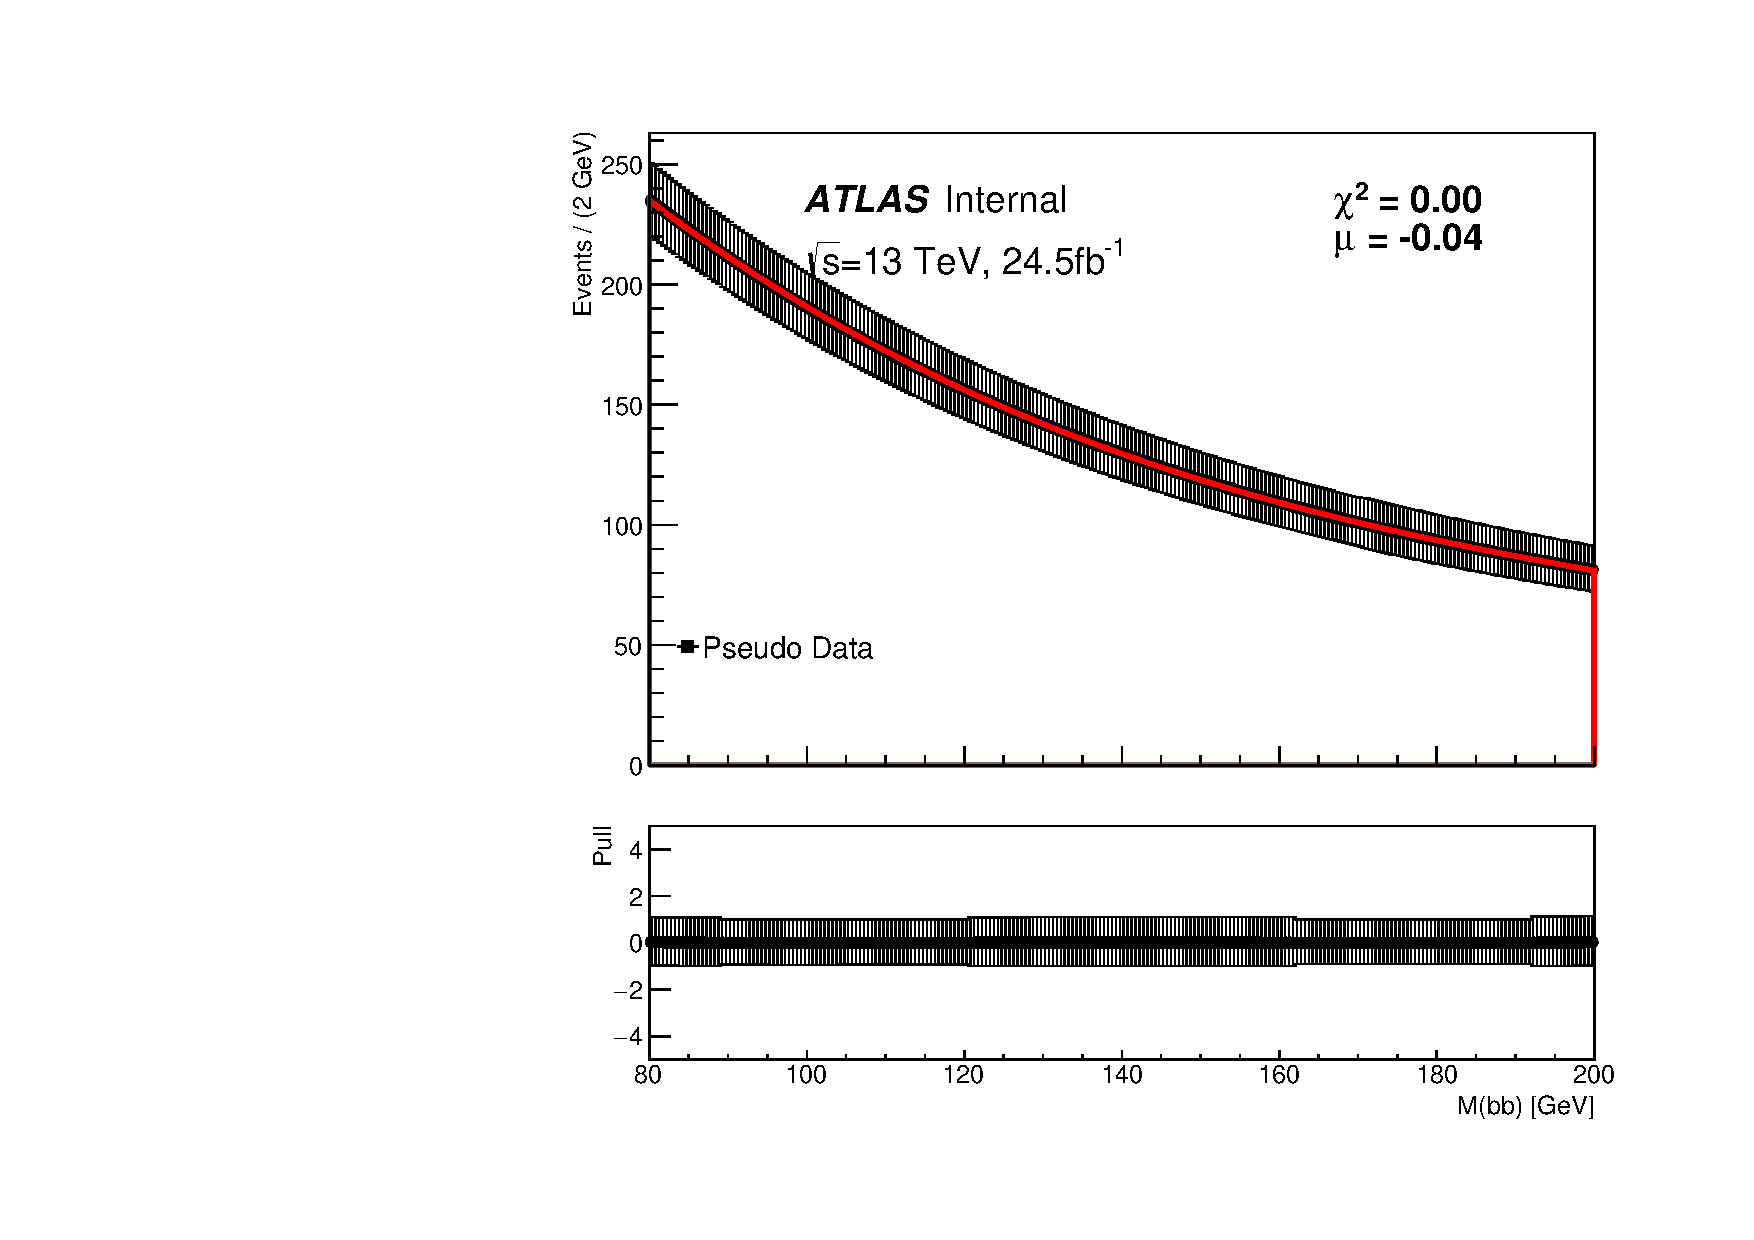
\includegraphics[width=0.24\textwidth]{figures/VBF/Spurious_ExpoO2_testVBF_ICHEP_4cen_SRI.pdf}
% 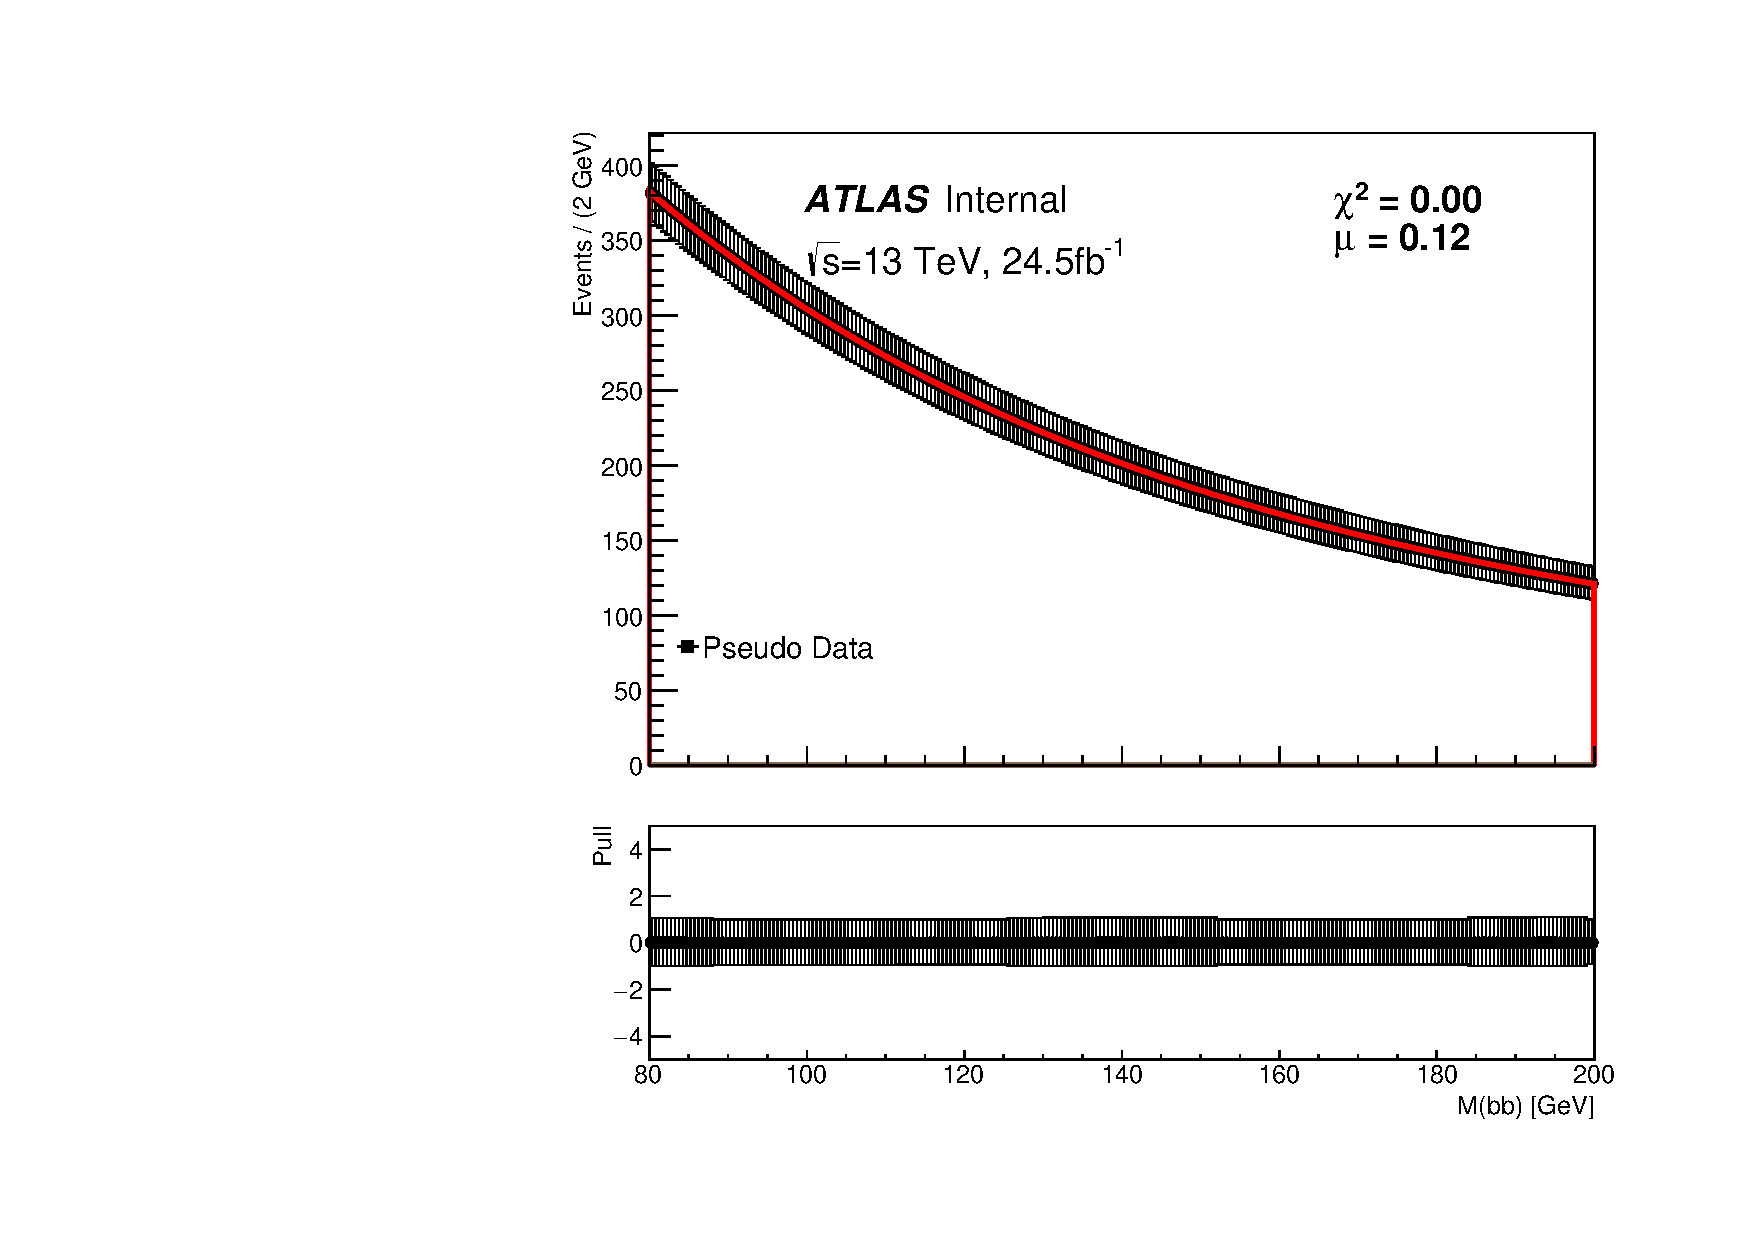
\includegraphics[width=0.24\textwidth]{figures/VBF/Spurious_ExpoO2_testVBF_ICHEP_4cen_SRII.pdf}
% 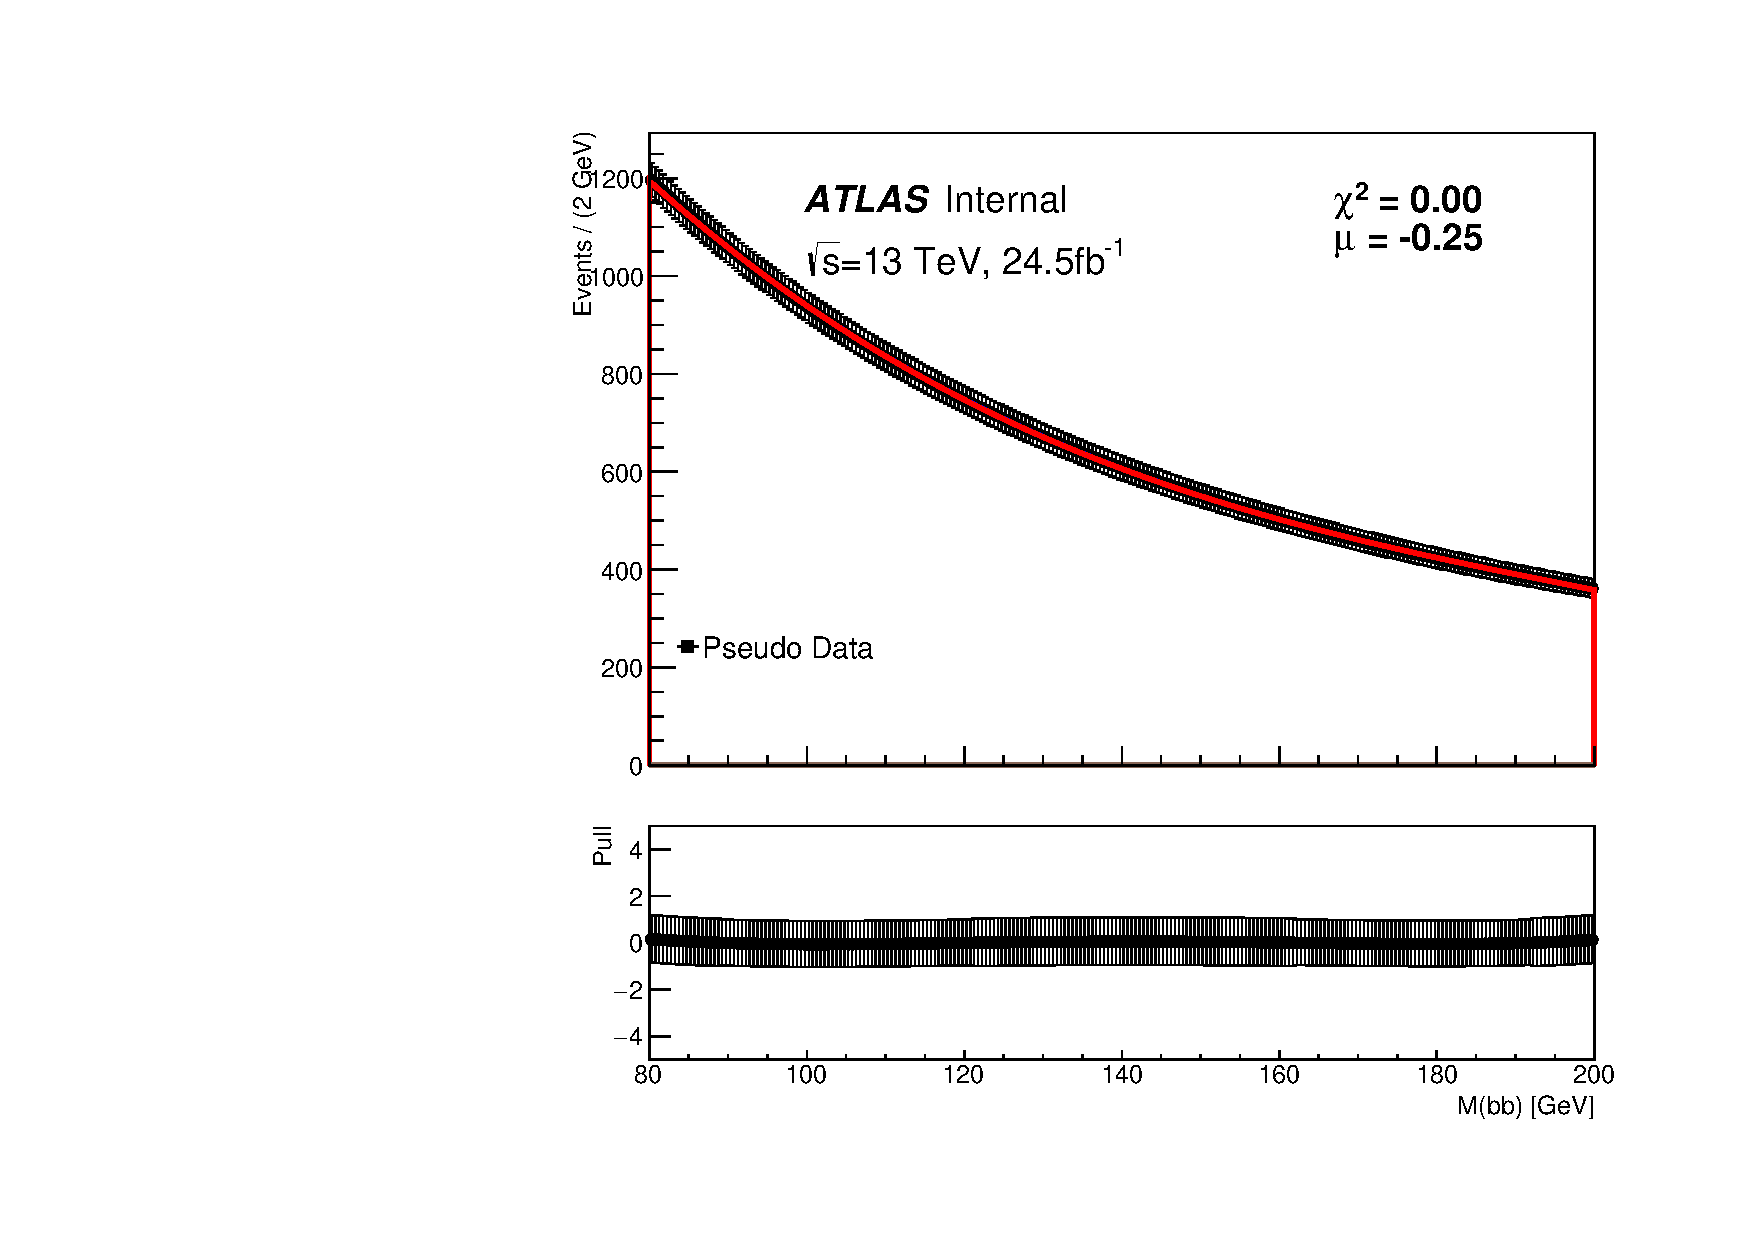
\includegraphics[width=0.24\textwidth]{figures/VBF/Spurious_ExpoO2_testVBF_ICHEP_4cen_SRIII.pdf}
% 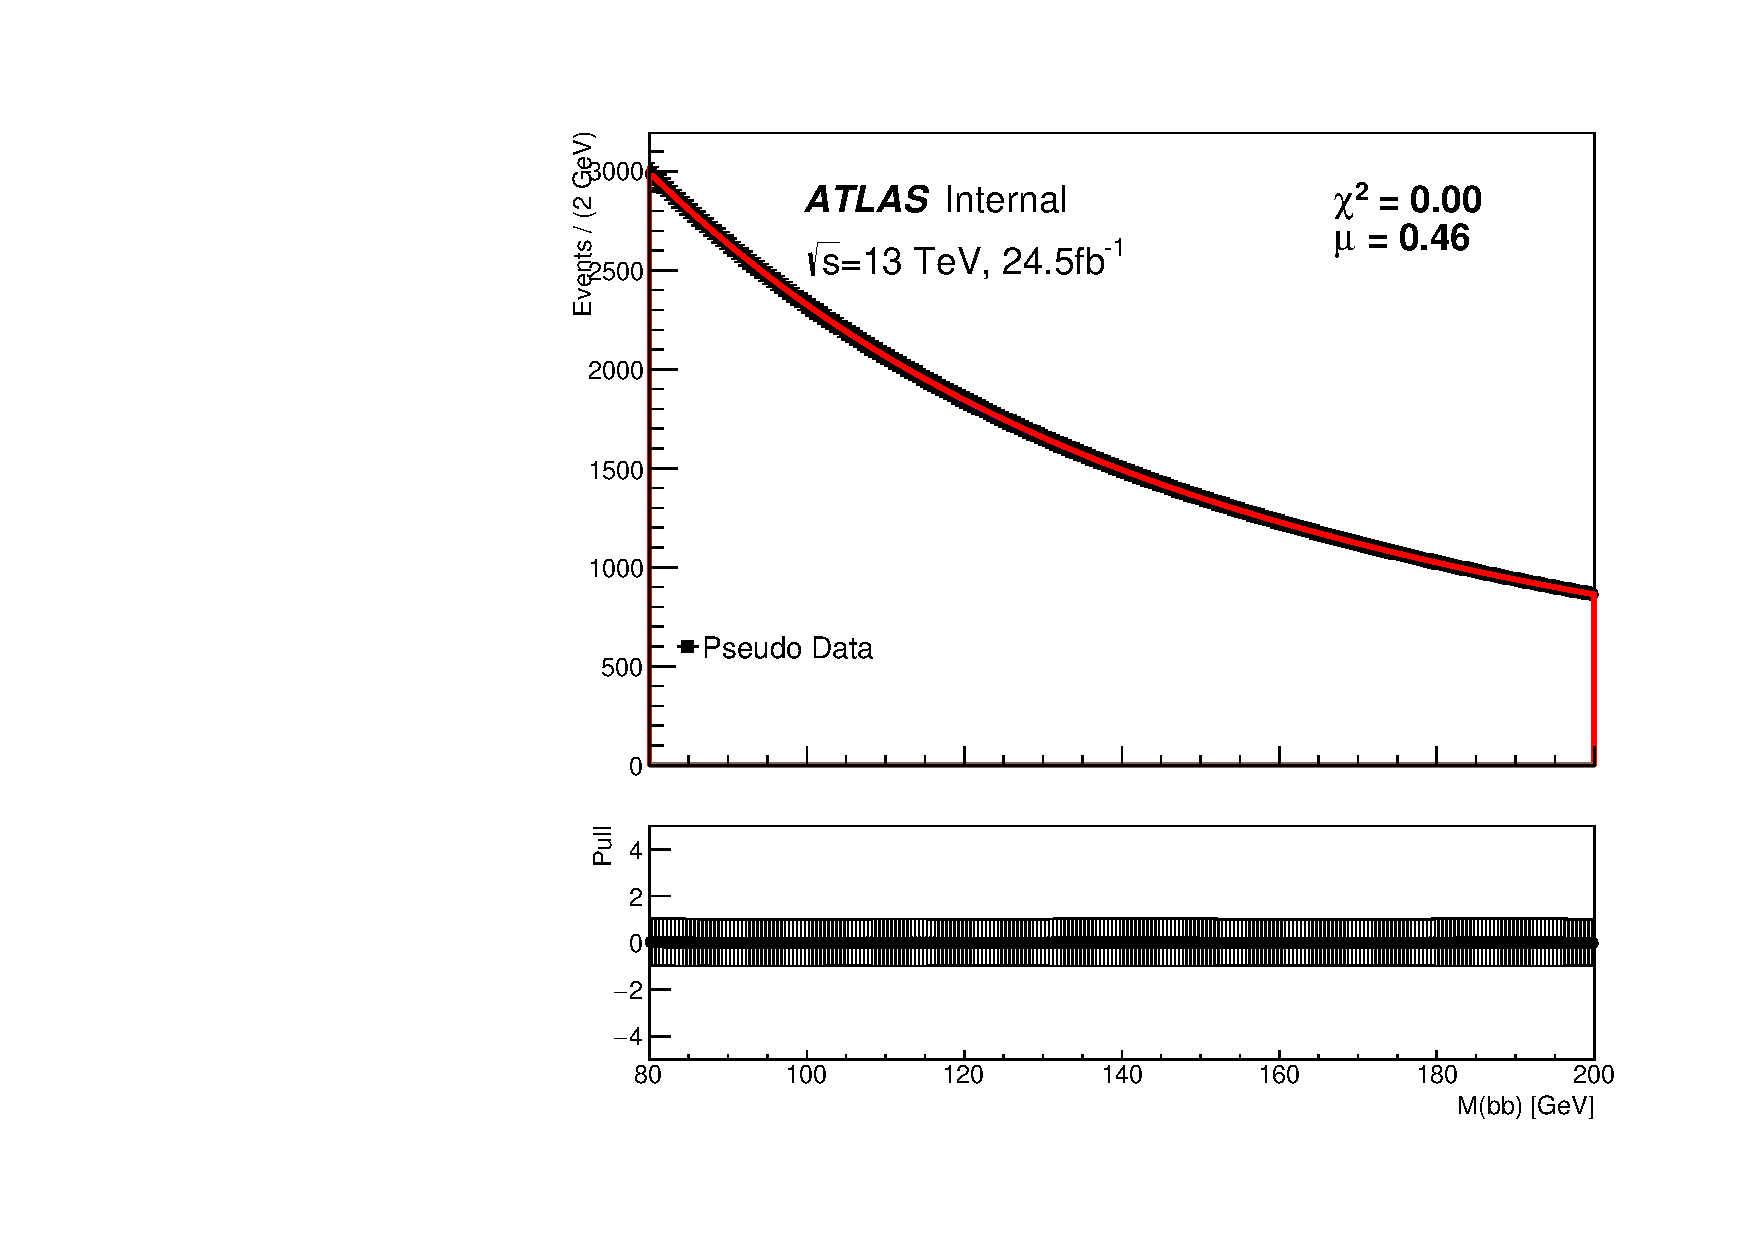
\includegraphics[width=0.24\textwidth]{figures/VBF/Spurious_ExpoO2_testVBF_ICHEP_4cen_SRIV.pdf}\\
% 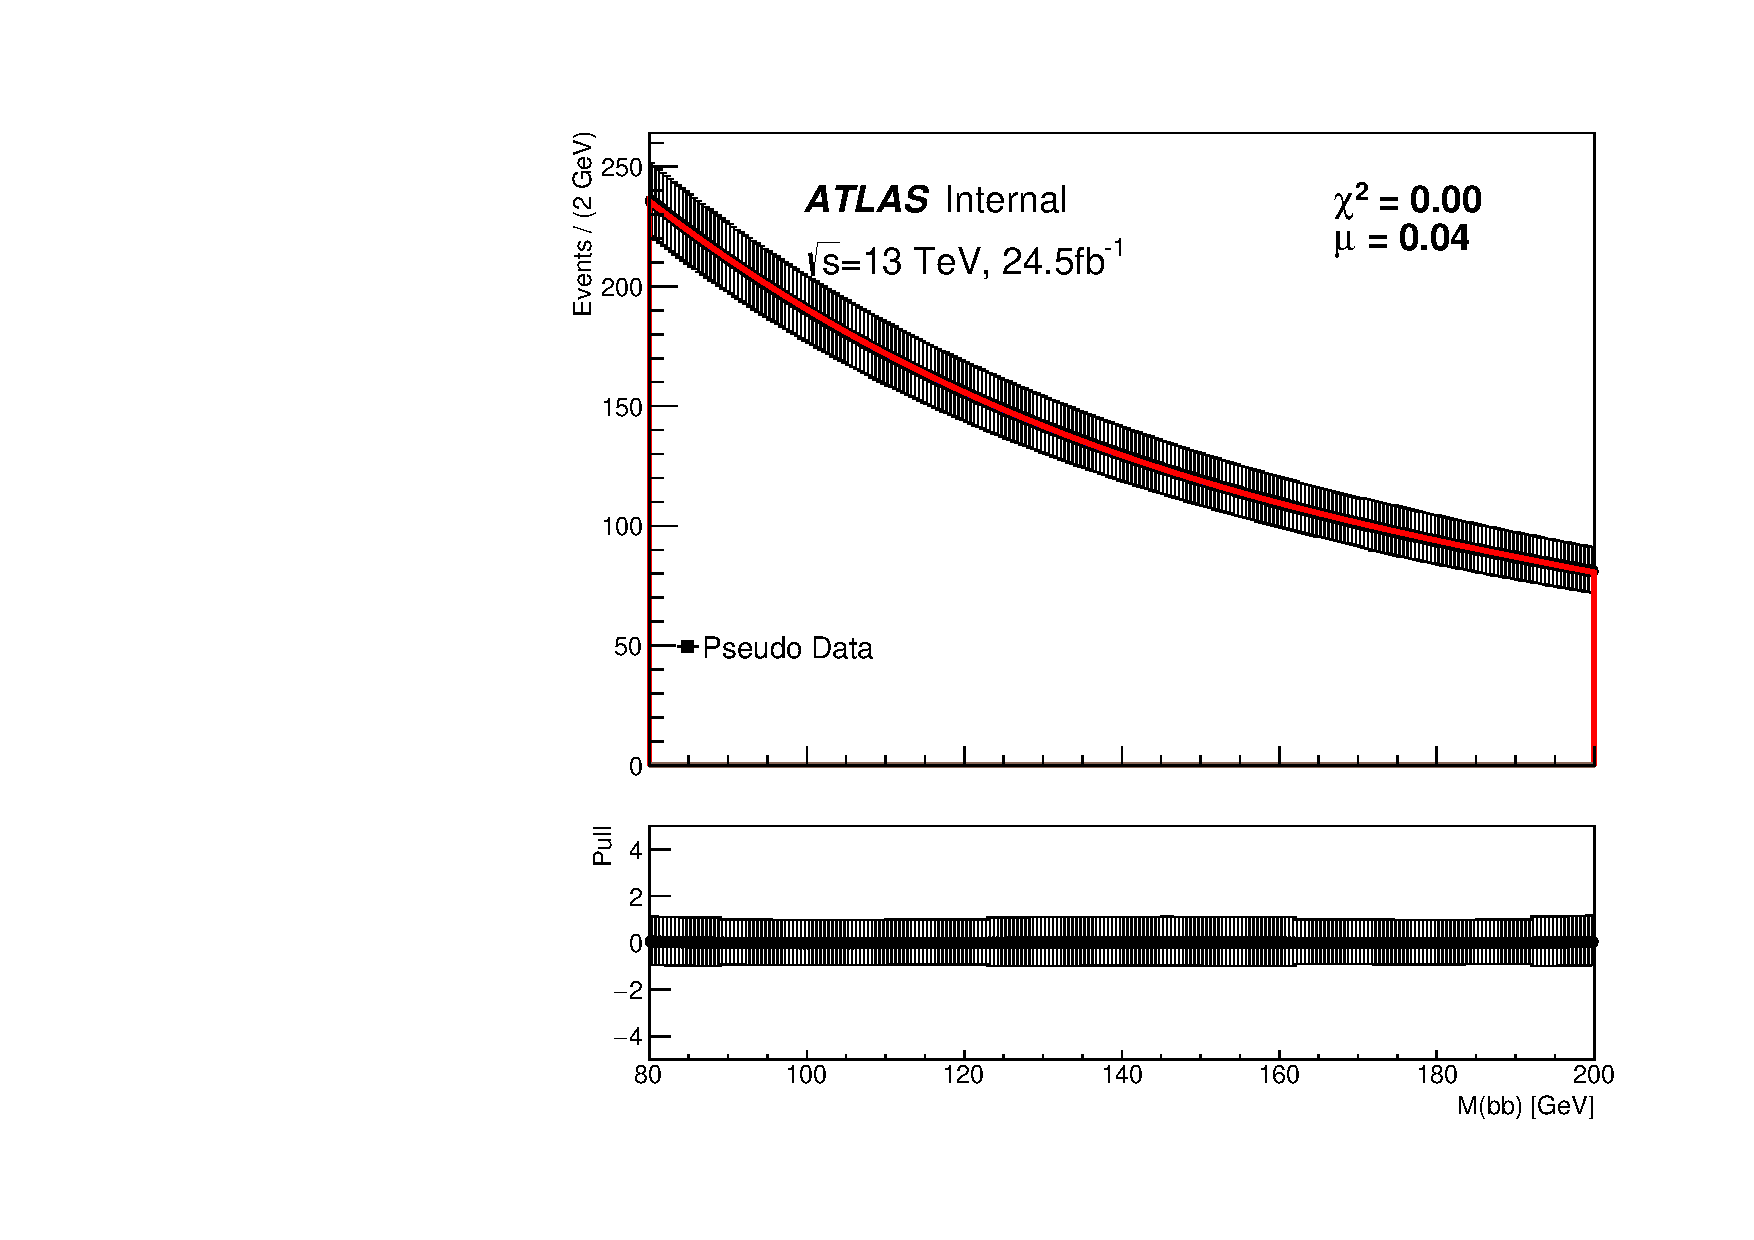
\includegraphics[width=0.24\textwidth]{figures/VBF/Spurious_SExpoO2_testVBF_ICHEP_4cen_SRI.pdf}
% 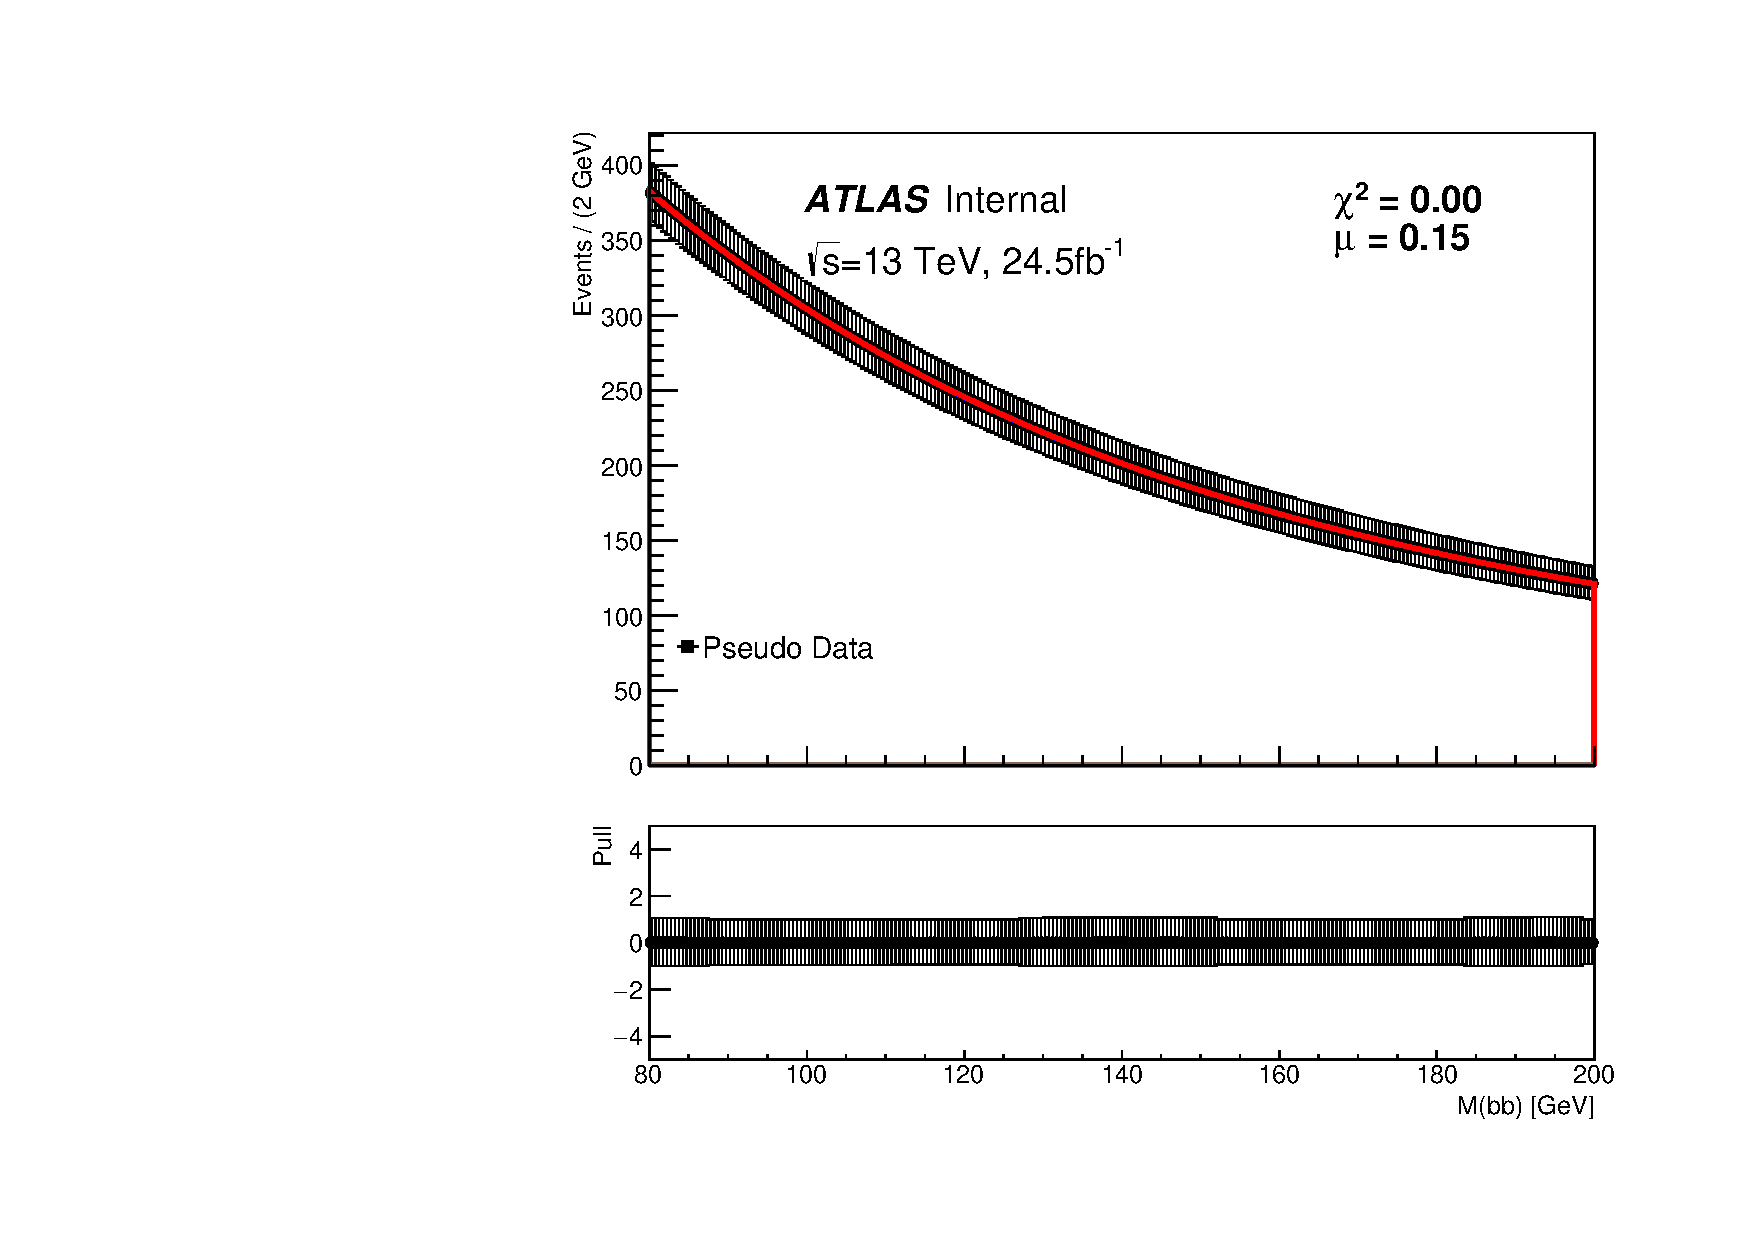
\includegraphics[width=0.24\textwidth]{figures/VBF/Spurious_SExpoO2_testVBF_ICHEP_4cen_SRII.pdf}
% 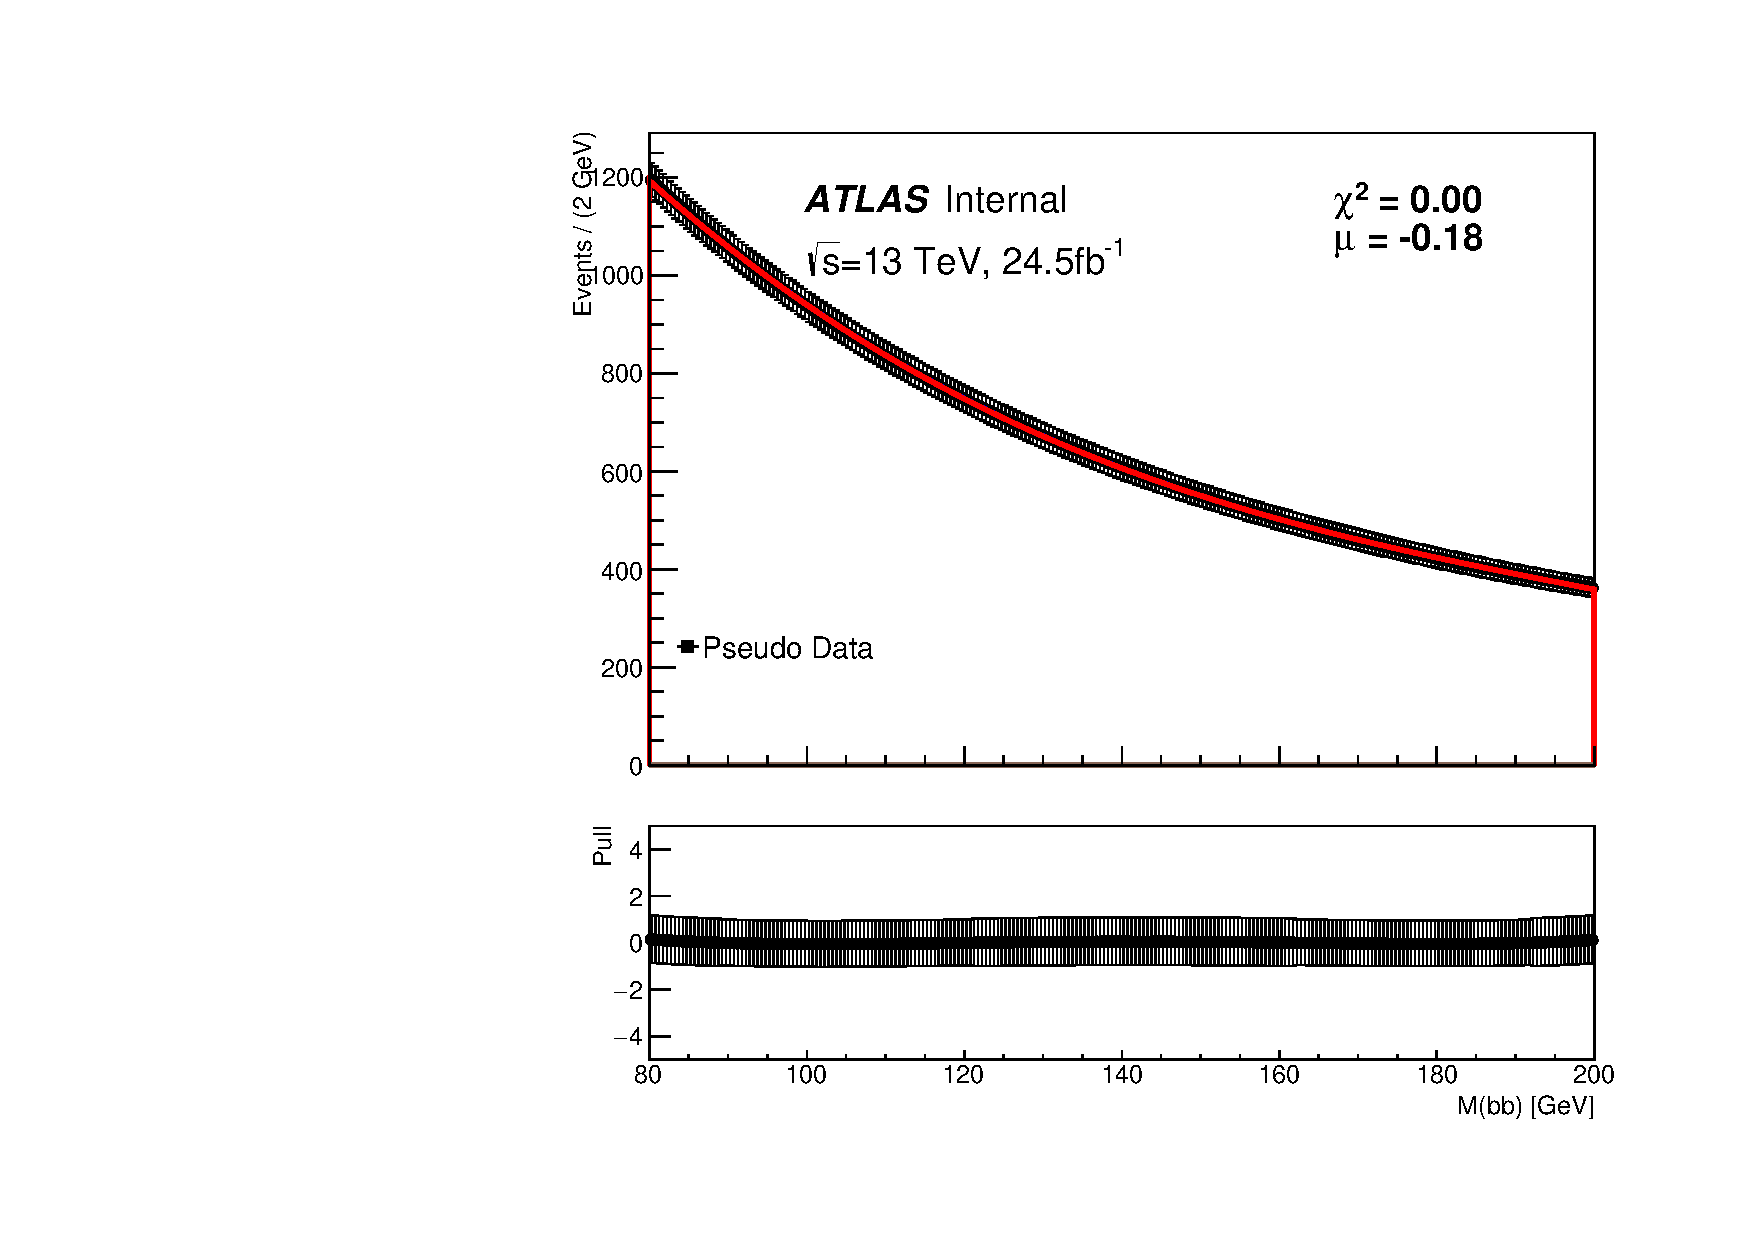
\includegraphics[width=0.24\textwidth]{figures/VBF/Spurious_SExpoO2_testVBF_ICHEP_4cen_SRIII.pdf}
% 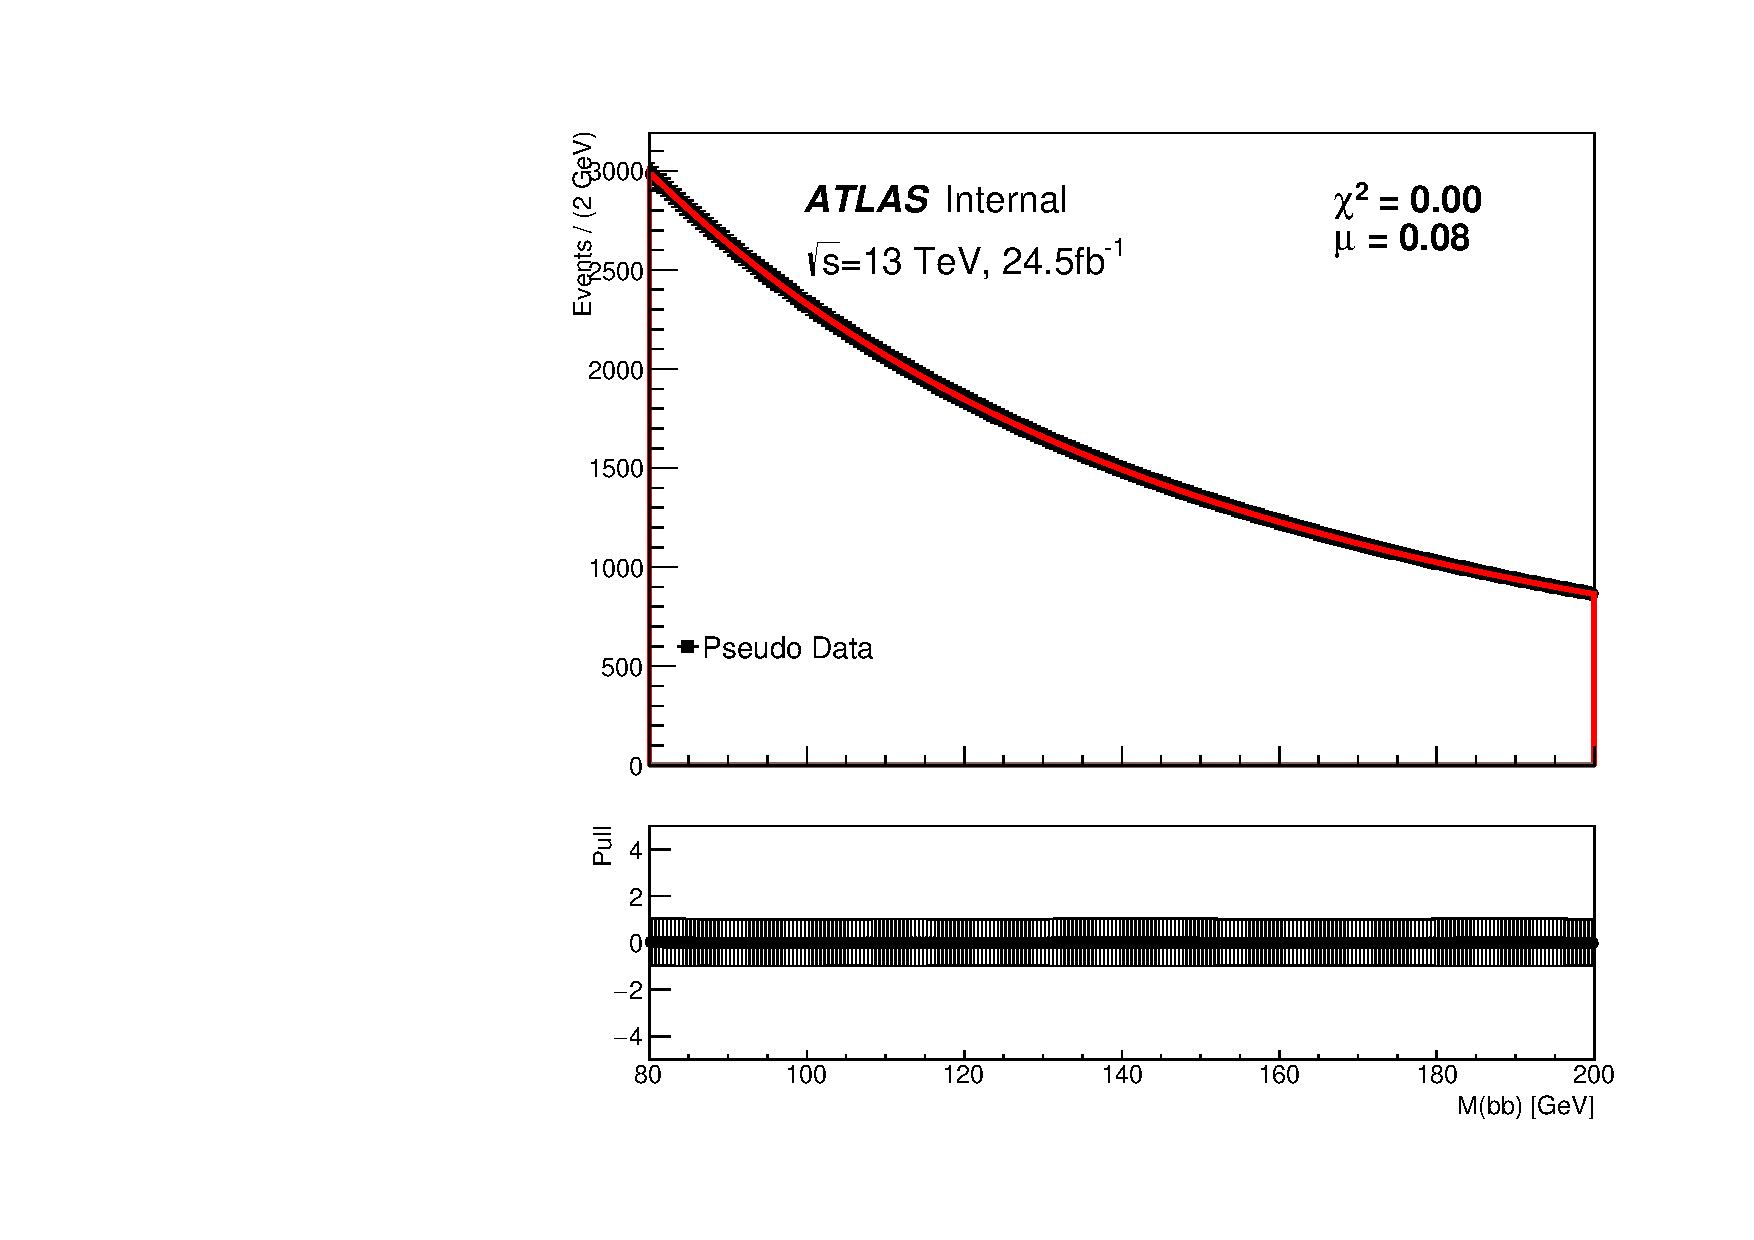
\includegraphics[width=0.24\textwidth]{figures/VBF/Spurious_SExpoO2_testVBF_ICHEP_4cen_SRIV.pdf}\\
%\caption{Spurious signal fit for \fourcentral channel for SR I to SR IV (from left to right). The best Bernstein background models are tested against alternative truth models Expo*Bernstein O(2) (top) and Sum of Expo O(2) (bottom).}
%  \label{fig:vbf-Fit_SP_4cen}
%\end{figure}



%\begin{table}[htbp]
%\centering
%\caption{Higgs sensitivity of each channel quantified in $\Delta \mu$ for different orders of non-resonant background function choice}
%\label{tab:perchannel_sensitivity}
%\begin{tabular}{|c|c|c|c|}
%\hline
%Channel      & Bernstein O2 & Bernstein O3 & Bernstein O4 \\ \hline
%2cen, SR I   & 2.09         & 2.67         &              \\ \hline
%2cen, SR II  & 5.50         & 8.09         &              \\ \hline
%4cen, SR I   & 2.86         & 3.60         &              \\ \hline
%4cen, SR II  & 6.44         & 9.32         & 10.07        \\ \hline
%4cen, SR III & 5.23         & 7.01         &              \\ \hline
%4cen, SR IV  & 4.20         & 5.51         & 5.89         \\ \hline
%\end{tabular}
%\end{table}

